%TC:incbib
%TC:macro \cite [option:text,text]
%TC:macro \citep [option:text,text]
%TC:macro \citet [option:text,text]
%TC:group table 0 1
%TC:group tabular 1 1

\section{Introduction}

At the very beginning of this thesis we would like to invite the reader to a little thought experiment. Imagine that you rely on a smart home system such as Google Home or Amazon Alexa for the safety of your house. What would you expect from your voice assistant to do when you say the following command:

"Hey Google, lock the door after I leave"

Probably exactly that, to lock the door, right? The following work will illustrate how a state-of-the-art machine learning model used in many systems including voice assistants, can be fooled with simple methods so that your front door will be open all day. 

With the integration of computer vision for self-driving cars, natural language processing for controlling our smart homes, and other applications of deep neural networks (DNN) in our daily lives, our reliance on technology increases and, with it, also the concerns about the security of neural networks. These security concerns grow as natural language processing (NLP) models are deployed in production systems such as fake news detectors, live translation, and speech recognition in voice assistants. NLP is a field of artificial intelligence that addresses the interaction between computers and humans using natural language.  
Szegedy et al. were the first in 2013 to find that minimal, and often imperceptible perturbations of the input data can fool a DNN into incorrect classifications \cite{szegedy2013intriguing}.
Adversarial examples are a way to highlight model vulnerabilities and are useful for the evaluation and interpretation of DNNs. 
Since the introduction of voice assistants on mobile devices like smartphones and home assistants, the research motivation to generate adversarial examples NLP has increased. Jia and Liang were the first to conduct adversarial attacks on textual DNNs and gained attention in the NLP community\cite{Jia2017AdversarialEF}. Since then, many studies have investigated the security of DNNs for NLP and proposed several attack methods for different target models. 

In 2018, Google AI researchers achieved a breakthrough in NLP by introducing BERT, a deep contextual language representation model that leverages transfer-learning by pre-training the model on large corpora with subsequent fine-tuning on a variety of downstream-tasks like text-classification, question answering, sentiment analysis, and more \cite{devlin2018bert}. To this day, BERT is state-of-the-art for many tasks in natural language processing and applied in various use-cases like automatic translation, google search requests, and voice assistant prompts. 
Given its increasing use in security-sensitive applications such as sentiment analysis and toxic content detection, it highly concerns that the BERT model's security vulnerabilities are still largely unknown and not a large field of research.

This thesis aims to explore the robustness of the BERT model used for Aspect-Based Sentiment Analysis (ABSA), a task in NLP. 


%-------------------------------------------------------------------
%-------------------------------------------------------------------
%-------------------Theoretical Background--------------------------
%-------------------------------------------------------------------
%-------------------------------------------------------------------

\section{Theoretical Background and Related Work}

In this section, we give an overview of the areas this thesis is build up on and the state of the art related to the respective research is outlined. First, the theoretical concepts of deep neural networks (DNN), NLP, and adversarial examples are explained. Secondly, we provide an overview of the proposed attacking methods on NLP to date. These concepts, combined with the review of related work, is used as a basis for the experiments conducted in the practical part of this thesis. 

%-------------------------------DNN---------------------------------
\subsection{Deep Learning}
The following chapter gives a brief overview of the key concepts of DNNs, which are the basis for the work at hand. In their book, Goodfellow et al. provide deep insights into the subject. Summarizing their work, we overview the most important terms and functionalities to provide a theoretical basis for the areas discussed in this thesis. For a complete introduction to the topic, we refer to the literature \cite{bengio2017deep}. 

\textbf{Deep Neural Networks}

Deep neural networks are neural networks inspired by the biological neural network of a human brain to learn from examples and build knowledge. 
DNNs perform a non-linear data transformation and can be used for multiple purposes, e.g., image-recognition, text-classification, audio-transcription, and more \cite{rawat2017deep}.
The input of a DNN consists of multiple data points transformed into a meaningful output by the model. The key concept is that the DNN learns the data distribution through self-found features.
In the training process of a DNN, a model is repeatedly fed with samples of a training-dataset $x \in X$ and the respective expected output $y$.

\textbf{The learning process}

Every neural network consists of an input, an output, and $1\dots n$ hidden layers, as illustrated in figure~\ref{fig:DNN}.
The input layer is the first layer of a network, which receives the input and forwards it to the intermediate, so-called hidden layers within the network. These layers perform non-linear transformations to the input to generate output which they pass on to the final layer of the network, the output layer. 
\begin{figure}
\centering
\tikzset{every picture/.style={line width=0.75pt}} %set default line width to 0.75pt
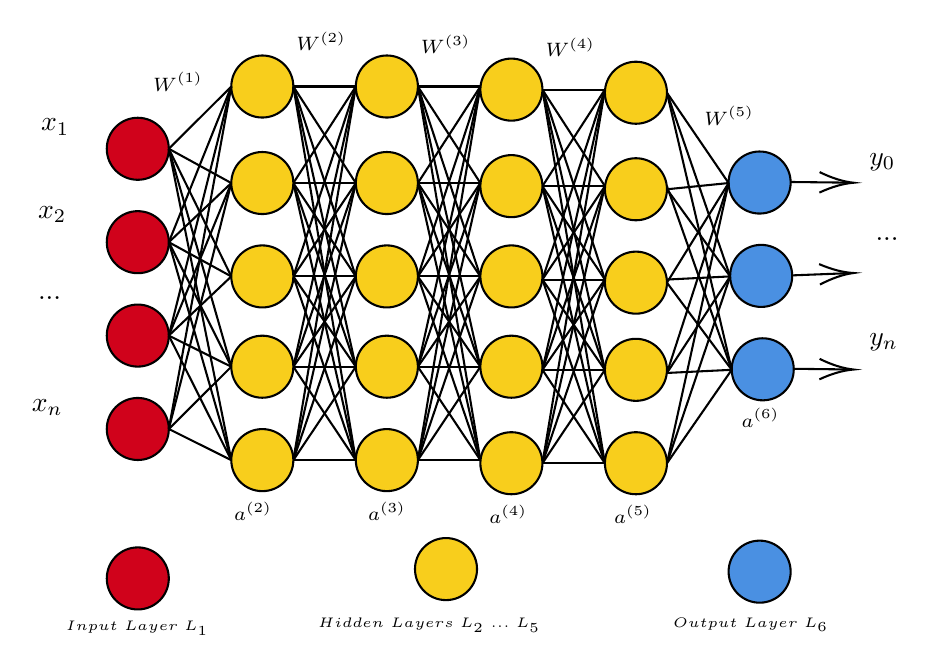
\begin{tikzpicture}[x=0.75pt,y=0.75pt,yscale=-1.5,xscale=1.5]
%uncomment if require: \path (0,341); %set diagram left start at 0, and has height of 341

%Shape: Circle [id:dp9036507142879056] 
\draw [fill={rgb, 255:red, 208; green, 2; blue, 27 } ,fill opacity=1 ] (112.07,69.97) .. controls (112.07,64.46) and (116.53,60) .. (122.03,60) .. controls (127.54,60) and (132,64.46) .. (132,69.97) .. controls (132,75.47) and (127.54,79.93) .. (122.03,79.93) .. controls (116.53,79.93) and (112.07,75.47) .. (112.07,69.97) -- cycle ;
%Shape: Circle [id:dp392140696827049] 
\draw [fill={rgb, 255:red, 208; green, 2; blue, 27 } ,fill opacity=1 ] (112.07,159.97) .. controls (112.07,154.46) and (116.53,150) .. (122.03,150) .. controls (127.54,150) and (132,154.46) .. (132,159.97) .. controls (132,165.47) and (127.54,169.93) .. (122.03,169.93) .. controls (116.53,169.93) and (112.07,165.47) .. (112.07,159.97) -- cycle ;
%Shape: Circle [id:dp5092562841379737] 
\draw [fill={rgb, 255:red, 208; green, 2; blue, 27 } ,fill opacity=1 ] (112.07,129.97) .. controls (112.07,124.46) and (116.53,120) .. (122.03,120) .. controls (127.54,120) and (132,124.46) .. (132,129.97) .. controls (132,135.47) and (127.54,139.93) .. (122.03,139.93) .. controls (116.53,139.93) and (112.07,135.47) .. (112.07,129.97) -- cycle ;
%Shape: Circle [id:dp741575646956142] 
\draw [fill={rgb, 255:red, 208; green, 2; blue, 27 } ,fill opacity=1 ] (112.07,99.97) .. controls (112.07,94.46) and (116.53,90) .. (122.03,90) .. controls (127.54,90) and (132,94.46) .. (132,99.97) .. controls (132,105.47) and (127.54,109.93) .. (122.03,109.93) .. controls (116.53,109.93) and (112.07,105.47) .. (112.07,99.97) -- cycle ;
%Shape: Circle [id:dp8747893475728183] 
\draw [fill={rgb, 255:red, 248; green, 206; blue, 28 } ,fill opacity=1 ] (152.07,49.97) .. controls (152.07,44.46) and (156.53,40) .. (162.03,40) .. controls (167.54,40) and (172,44.46) .. (172,49.97) .. controls (172,55.47) and (167.54,59.93) .. (162.03,59.93) .. controls (156.53,59.93) and (152.07,55.47) .. (152.07,49.97) -- cycle ;
%Straight Lines [id:da7388391985482041] 
\draw [line width=0.75]  (132,69.97) -- (152.07,49.97) ;
%Straight Lines [id:da07594424125920374] 
\draw [line width=0.75]  (132,69.97) -- (152.07,80.97) ;
%Straight Lines [id:da32078114159480653] 
\draw [line width=0.75]    (132,69.97) -- (152.07,110.97) ;
%Straight Lines [id:da6110475522563447] 
\draw [line width=0.75]    (132,69.97) -- (152.07,139.97) ;
%Straight Lines [id:da041179344816883456] 
\draw [line width=0.75]    (132,69.97) -- (152.07,169.97) ;
%Straight Lines [id:da2602448175108121] 
\draw [line width=0.75]    (132,99.97) -- (152.07,49.97) ;
%Straight Lines [id:da008093692172857048] 
\draw [line width=0.75]    (132,129.97) -- (152.07,80.97) ;
%Straight Lines [id:da6407207321117384] 
\draw    (132,99.97) -- (152.07,110.97) ;
%Straight Lines [id:da14218645121820817] 
\draw    (132,99.97) -- (152.07,139.97) ;
%Straight Lines [id:da5086959379820909] 
\draw    (132,99.97) -- (152.07,169.97) ;
%Straight Lines [id:da27535229192580724] 
\draw    (132,129.97) -- (152.07,49.97) ;
%Straight Lines [id:da14037699589827302] 
\draw    (132,129.97) -- (152.07,110.97) ;
%Straight Lines [id:da0004577781898109645] 
\draw    (132,129.97) -- (152.07,139.97) ;
%Straight Lines [id:da021283898277069335] 
\draw    (132,129.97) -- (152.07,169.97) ;
%Straight Lines [id:da11277756016216589] 
\draw    (132,159.97) -- (152.07,169.97) ;
%Straight Lines [id:da07695362342089163] 
\draw    (132,159.97) -- (152.07,139.97) ;
%Straight Lines [id:da7003177955335873] 
\draw    (132,159.97) -- (152.07,80.97) ;
%Straight Lines [id:da13003755544947393] 
\draw    (132,159.97) -- (152.07,49.97) ;
%Straight Lines [id:da0258965022860157] 
\draw    (132,99.97) -- (152.07,80.97) ;
%Straight Lines [id:da5272455432469216] 
\draw    (172,49.97) -- (192.07,49.97) ;
%Straight Lines [id:da7176795652766319] 
\draw    (192.07,80.97) -- (172,49.97) ;
%Straight Lines [id:da44709081360312275] 
\draw    (192.07,110.97) -- (172,49.97) ;
%Straight Lines [id:da5060111738899119] 
\draw    (192.07,139.97) -- (172,49.97) ;
%Straight Lines [id:da18932391727567288] 
\draw    (192.07,169.97) -- (172,49.97) ;
%Straight Lines [id:da22011251193586712] 
\draw    (192.07,49.97) -- (172,80.97) ;
%Straight Lines [id:da28163631108589815] 
\draw    (192.07,80.97) -- (172,80.97) ;
%Straight Lines [id:da8595703022713812] 
\draw    (192.07,110.97) -- (172,80.97) ;
%Straight Lines [id:da8985095100702133] 
\draw    (192.07,139.97) -- (172,80.97) ;
%Straight Lines [id:da2411640053472085] 
\draw    (192.07,169.97) -- (172,80.97) ;
%Straight Lines [id:da8971565419225193] 
\draw    (192.07,49.97) -- (172,110.97) ;
%Straight Lines [id:da43547451815310456] 
\draw    (192.07,80.97) -- (172,110.97) ;
%Straight Lines [id:da8113804544355533] 
\draw    (192.07,110.97) -- (172,110.97) ;
%Straight Lines [id:da023773670154593307] 
\draw    (192.07,139.97) -- (172,110.97) ;
%Straight Lines [id:da29220340496627095] 
\draw    (192.07,169.97) -- (172,110.97) ;
%Straight Lines [id:da46359790510412235] 
\draw    (192.07,49.97) -- (172,139.97) ;
%Straight Lines [id:da5966045171406014] 
\draw    (192.07,80.97) -- (172,139.97) ;
%Straight Lines [id:da1384195920973581] 
\draw    (192.07,110.97) -- (172,139.97) ;
%Straight Lines [id:da3215894260857254] 
\draw    (192.07,139.97) -- (172,139.97) ;
%Straight Lines [id:da8400489001252476] 
\draw    (192.07,169.97) -- (172,139.97) ;
%Straight Lines [id:da3221803153234972] 
\draw    (192.07,49.97) -- (172,169.97) ;
%Straight Lines [id:da7688605830945641] 
\draw    (192.07,80.97) -- (172,169.97) ;
%Straight Lines [id:da9165480220941868] 
\draw    (192.07,110.97) -- (172,169.97) ;
%Straight Lines [id:da3215336892666468] 
\draw    (192.07,139.97) -- (172,169.97) ;
%Straight Lines [id:da5525341830680578] 
\draw    (192.07,169.97) -- (172,169.97) ;
%Straight Lines [id:da1261118309670728] 
\draw    (212,49.97) -- (232.07,49.97) ;
%Straight Lines [id:da11900162455233043] 
\draw    (232.07,80.97) -- (212,49.97) ;
%Straight Lines [id:da5368627726392105] 
\draw    (232.07,110.97) -- (212,49.97) ;
%Straight Lines [id:da8605152876282114] 
\draw    (232.07,139.97) -- (212,49.97) ;
%Straight Lines [id:da4815832562914505] 
\draw    (232.07,169.97) -- (212,49.97) ;
%Straight Lines [id:da17003748064618818] 
\draw    (232.07,49.97) -- (212,80.97) ;
%Straight Lines [id:da1480484348333101] 
\draw    (232.07,80.97) -- (212,80.97) ;
%Straight Lines [id:da2124086159740538] 
\draw    (232.07,110.97) -- (212,80.97) ;
%Straight Lines [id:da8479733865567239] 
\draw    (232.07,139.97) -- (212,80.97) ;
%Straight Lines [id:da5278087829516401] 
\draw    (232.07,169.97) -- (212,80.97) ;
%Straight Lines [id:da31210020478505274] 
\draw    (232.07,49.97) -- (212,110.97) ;
%Straight Lines [id:da8124121959107438] 
\draw    (232.07,80.97) -- (212,110.97) ;
%Straight Lines [id:da7256728672602327] 
\draw    (232.07,110.97) -- (212,110.97) ;
%Straight Lines [id:da4579977059630831] 
\draw    (232.07,139.97) -- (212,110.97) ;
%Straight Lines [id:da4553391144095986] 
\draw    (232.07,169.97) -- (212,110.97) ;
%Straight Lines [id:da7122744544190456] 
\draw    (232.07,49.97) -- (212,139.97) ;
%Straight Lines [id:da8556567438522781] 
\draw    (232.07,80.97) -- (212,139.97) ;
%Straight Lines [id:da4566333841323885] 
\draw    (232.07,110.97) -- (212,139.97) ;
%Straight Lines [id:da5987581471646565] 
\draw    (232.07,139.97) -- (212,139.97) ;
%Straight Lines [id:da6269621991811268] 
\draw    (232.07,169.97) -- (212,139.97) ;
%Straight Lines [id:da6451496592431717] 
\draw    (232.07,49.97) -- (212,169.97) ;
%Straight Lines [id:da1496571288127746] 
\draw    (232.07,80.97) -- (212,169.97) ;
%Straight Lines [id:da9155668903600209] 
\draw    (232.07,110.97) -- (212,169.97) ;
%Straight Lines [id:da7832007038396517] 
\draw    (232.07,139.97) -- (212,169.97) ;
%Straight Lines [id:da6430768734831682] 
\draw    (232.07,169.97) -- (212,169.97) ;
%Straight Lines [id:da502353093987252] 
\draw    (252,50.97) -- (272.07,50.97) ;
%Straight Lines [id:da962031096991036] 
\draw    (272.07,81.97) -- (252,50.97) ;
%Straight Lines [id:da269614537255464] 
\draw    (272.07,111.97) -- (252,50.97) ;
%Straight Lines [id:da06353430327255638] 
\draw    (272.07,140.97) -- (252,50.97) ;
%Straight Lines [id:da13730470406815432] 
\draw    (272.07,170.97) -- (252,50.97) ;
%Straight Lines [id:da4524270736830083] 
\draw    (272.07,50.97) -- (252,81.97) ;
%Straight Lines [id:da9801938127403164] 
\draw    (272.07,81.97) -- (252,81.97) ;
%Straight Lines [id:da15200177386551716] 
\draw    (272.07,111.97) -- (252,81.97) ;
%Straight Lines [id:da819342894818783] 
\draw    (272.07,140.97) -- (252,81.97) ;
%Straight Lines [id:da961969476032104] 
\draw    (272.07,170.97) -- (252,81.97) ;
%Straight Lines [id:da4605571032482948] 
\draw    (272.07,50.97) -- (252,111.97) ;
%Straight Lines [id:da3325926047277312] 
\draw    (272.07,81.97) -- (252,111.97) ;
%Straight Lines [id:da9190202484946008] 
\draw    (272.07,111.97) -- (252,111.97) ;
%Straight Lines [id:da5757807552216108] 
\draw    (272.07,140.97) -- (252,111.97) ;
%Straight Lines [id:da31627284665396105] 
\draw    (272.07,170.97) -- (252,111.97) ;
%Straight Lines [id:da3543230253141595] 
\draw    (272.07,50.97) -- (252,140.97) ;
%Straight Lines [id:da9638413022900825] 
\draw    (272.07,81.97) -- (252,140.97) ;
%Straight Lines [id:da5744945840591497] 
\draw    (272.07,111.97) -- (252,140.97) ;
%Straight Lines [id:da46298335493097875] 
\draw    (272.07,140.97) -- (252,140.97) ;
%Straight Lines [id:da963474757022725] 
\draw    (272.07,170.97) -- (252,140.97) ;
%Straight Lines [id:da6330401371775292] 
\draw    (272.07,50.97) -- (252,170.97) ;
%Straight Lines [id:da5996286002388257] 
\draw    (272.07,81.97) -- (252,170.97) ;
%Straight Lines [id:da412529317044946] 
\draw    (272.07,111.97) -- (252,170.97) ;
%Straight Lines [id:da6167493426794559] 
\draw    (272.07,140.97) -- (252,170.97) ;
%Straight Lines [id:da9155797500498795] 
\draw    (272.07,170.97) -- (252,170.97) ;
%Shape: Circle [id:dp9260210835392857] 
\draw  [fill={rgb, 255:red, 74; green, 144; blue, 226 }  ,fill opacity=1 ] (332.73,140.63) .. controls (332.83,146.13) and (328.44,150.67) .. (322.94,150.76) .. controls (317.43,150.85) and (312.9,146.46) .. (312.8,140.96) .. controls (312.71,135.46) and (317.1,130.92) .. (322.6,130.83) .. controls (328.11,130.74) and (332.64,135.12) .. (332.73,140.63) -- cycle ;
%Shape: Circle [id:dp4331085521150484] 
\draw  [fill={rgb, 255:red, 74; green, 144; blue, 226 }  ,fill opacity=1 ] (331.73,80.63) .. controls (331.82,86.14) and (327.43,90.67) .. (321.93,90.77) .. controls (316.43,90.86) and (311.89,86.47) .. (311.8,80.97) .. controls (311.71,75.46) and (316.09,70.93) .. (321.6,70.84) .. controls (327.1,70.74) and (331.64,75.13) .. (331.73,80.63) -- cycle ;
%Shape: Circle [id:dp3743672592545707] 
\draw  [fill={rgb, 255:red, 74; green, 144; blue, 226 }  ,fill opacity=1 ] (332.23,110.63) .. controls (332.32,116.13) and (327.94,120.67) .. (322.43,120.76) .. controls (316.93,120.85) and (312.39,116.47) .. (312.3,110.96) .. controls (312.21,105.46) and (316.6,100.92) .. (322.1,100.83) .. controls (327.6,100.74) and (332.14,105.13) .. (332.23,110.63) -- cycle ;
%Straight Lines [id:da1506829248270687] 
\draw    (292,51.97) -- (311.8,80.97) ;
%Straight Lines [id:da3048311510472882] 
\draw    (292,51.97) -- (312.3,110.96) ;
%Straight Lines [id:da15082332561192868] 
\draw    (292,51.97) -- (312.8,140.96) ;
%Straight Lines [id:da16040780327570636] 
\draw    (292,82.97) -- (311.8,80.97) ;
%Straight Lines [id:da21903521854428198] 
\draw    (292,112.97) -- (311.8,80.97) ;
%Straight Lines [id:da5012655564753412] 
\draw    (292,111.97) -- (312.3,110.96) ;
%Straight Lines [id:da7219622968472209] 
\draw    (292,112.97) -- (312.8,140.96) ;
%Straight Lines [id:da9995650526933821] 
\draw    (292,141.97) -- (311.8,80.97) ;
%Straight Lines [id:da3902600091687223] 
\draw    (292,141.97) -- (312.3,110.96) ;
%Straight Lines [id:da2503346740038974] 
\draw    (292,141.97) -- (312.8,140.96) ;
%Straight Lines [id:da19110169967835922] 
\draw    (292,170.97) -- (312.8,140.96) ;
%Straight Lines [id:da663166954945558] 
\draw    (292,170.97) -- (312.3,110.96) ;
%Straight Lines [id:da03383526862017594] 
\draw    (292,170.97) -- (311.8,80.97) ;
%Straight Lines [id:da304205093315273] 
\draw    (292,82.97) -- (312.3,110.96) ;
%Straight Lines [id:da6109581685450142] 
\draw    (292,81.97) -- (312.8,140.96) ;
%Straight Lines [id:da48761809810505297] 
\draw    (331.73,80.63) -- (349.93,80.84) ;
\draw [shift={(351.93,80.87)}, rotate = 180.66] [color={rgb, 255:red, 0; green, 0; blue, 0 }  ][line width=0.75]    (10.93,-3.29) .. controls (6.95,-1.4) and (3.31,-0.3) .. (0,0) .. controls (3.31,0.3) and (6.95,1.4) .. (10.93,3.29)   ;
%Straight Lines [id:da8815522416855154] 
\draw    (332.73,140.63) -- (349.93,140.84) ;
\draw [shift={(351.93,140.87)}, rotate = 180.72] [color={rgb, 255:red, 0; green, 0; blue, 0 }  ][line width=0.75]    (10.93,-3.29) .. controls (6.95,-1.4) and (3.31,-0.3) .. (0,0) .. controls (3.31,0.3) and (6.95,1.4) .. (10.93,3.29)   ;
%Straight Lines [id:da24476421235573498] 
\draw    (332.23,110.63) -- (349.93,109.94) ;
\draw [shift={(351.93,109.87)}, rotate = 537.78] [color={rgb, 255:red, 0; green, 0; blue, 0 }  ][line width=0.75]    (10.93,-3.29) .. controls (6.95,-1.4) and (3.31,-0.3) .. (0,0) .. controls (3.31,0.3) and (6.95,1.4) .. (10.93,3.29)   ;
%Shape: Circle [id:dp0647726642351596] 
\draw  [fill={rgb, 255:red, 248; green, 206; blue, 28 }  ,fill opacity=1 ] (152.07,110.97) .. controls (152.07,105.46) and (156.53,101) .. (162.03,101) .. controls (167.54,101) and (172,105.46) .. (172,110.97) .. controls (172,116.47) and (167.54,120.93) .. (162.03,120.93) .. controls (156.53,120.93) and (152.07,116.47) .. (152.07,110.97) -- cycle ;
%Shape: Circle [id:dp263590793349345] 
\draw  [fill={rgb, 255:red, 248; green, 206; blue, 28 }  ,fill opacity=1 ] (152.07,80.97) .. controls (152.07,75.46) and (156.53,71) .. (162.03,71) .. controls (167.54,71) and (172,75.46) .. (172,80.97) .. controls (172,86.47) and (167.54,90.93) .. (162.03,90.93) .. controls (156.53,90.93) and (152.07,86.47) .. (152.07,80.97) -- cycle ;
%Shape: Circle [id:dp823583650983651] 
\draw  [fill={rgb, 255:red, 248; green, 206; blue, 28 }  ,fill opacity=1 ] (152.07,139.97) .. controls (152.07,134.46) and (156.53,130) .. (162.03,130) .. controls (167.54,130) and (172,134.46) .. (172,139.97) .. controls (172,145.47) and (167.54,149.93) .. (162.03,149.93) .. controls (156.53,149.93) and (152.07,145.47) .. (152.07,139.97) -- cycle ;
%Shape: Circle [id:dp836132286733146] 
\draw  [fill={rgb, 255:red, 248; green, 206; blue, 28 }  ,fill opacity=1 ] (152.07,169.97) .. controls (152.07,164.46) and (156.53,160) .. (162.03,160) .. controls (167.54,160) and (172,164.46) .. (172,169.97) .. controls (172,175.47) and (167.54,179.93) .. (162.03,179.93) .. controls (156.53,179.93) and (152.07,175.47) .. (152.07,169.97) -- cycle ;
%Shape: Circle [id:dp5221253594199046] 
\draw  [fill={rgb, 255:red, 248; green, 206; blue, 28 }  ,fill opacity=1 ] (192.07,49.97) .. controls (192.07,44.46) and (196.53,40) .. (202.03,40) .. controls (207.54,40) and (212,44.46) .. (212,49.97) .. controls (212,55.47) and (207.54,59.93) .. (202.03,59.93) .. controls (196.53,59.93) and (192.07,55.47) .. (192.07,49.97) -- cycle ;
%Shape: Circle [id:dp4183656064918385] 
\draw  [fill={rgb, 255:red, 248; green, 206; blue, 28 }  ,fill opacity=1 ] (192.07,80.97) .. controls (192.07,75.46) and (196.53,71) .. (202.03,71) .. controls (207.54,71) and (212,75.46) .. (212,80.97) .. controls (212,86.47) and (207.54,90.93) .. (202.03,90.93) .. controls (196.53,90.93) and (192.07,86.47) .. (192.07,80.97) -- cycle ;
%Shape: Circle [id:dp017558394040142034] 
\draw  [fill={rgb, 255:red, 248; green, 206; blue, 28 }  ,fill opacity=1 ] (192.07,110.97) .. controls (192.07,105.46) and (196.53,101) .. (202.03,101) .. controls (207.54,101) and (212,105.46) .. (212,110.97) .. controls (212,116.47) and (207.54,120.93) .. (202.03,120.93) .. controls (196.53,120.93) and (192.07,116.47) .. (192.07,110.97) -- cycle ;
%Shape: Circle [id:dp792774082065314] 
\draw  [fill={rgb, 255:red, 248; green, 206; blue, 28 }  ,fill opacity=1 ] (192.07,139.97) .. controls (192.07,134.46) and (196.53,130) .. (202.03,130) .. controls (207.54,130) and (212,134.46) .. (212,139.97) .. controls (212,145.47) and (207.54,149.93) .. (202.03,149.93) .. controls (196.53,149.93) and (192.07,145.47) .. (192.07,139.97) -- cycle ;
%Shape: Circle [id:dp97036578695106] 
\draw  [fill={rgb, 255:red, 248; green, 206; blue, 28 }  ,fill opacity=1 ] (192.07,169.97) .. controls (192.07,164.46) and (196.53,160) .. (202.03,160) .. controls (207.54,160) and (212,164.46) .. (212,169.97) .. controls (212,175.47) and (207.54,179.93) .. (202.03,179.93) .. controls (196.53,179.93) and (192.07,175.47) .. (192.07,169.97) -- cycle ;
%Shape: Circle [id:dp9155429880019643] 
\draw  [fill={rgb, 255:red, 248; green, 206; blue, 28 }  ,fill opacity=1 ] (232.07,50.97) .. controls (232.07,45.46) and (236.53,41) .. (242.03,41) .. controls (247.54,41) and (252,45.46) .. (252,50.97) .. controls (252,56.47) and (247.54,60.93) .. (242.03,60.93) .. controls (236.53,60.93) and (232.07,56.47) .. (232.07,50.97) -- cycle ;
%Shape: Circle [id:dp6266987748087688] 
\draw  [fill={rgb, 255:red, 248; green, 206; blue, 28 }  ,fill opacity=1 ] (232.07,81.97) .. controls (232.07,76.46) and (236.53,72) .. (242.03,72) .. controls (247.54,72) and (252,76.46) .. (252,81.97) .. controls (252,87.47) and (247.54,91.93) .. (242.03,91.93) .. controls (236.53,91.93) and (232.07,87.47) .. (232.07,81.97) -- cycle ;
%Shape: Circle [id:dp8021117419800181] 
\draw  [fill={rgb, 255:red, 248; green, 206; blue, 28 }  ,fill opacity=1 ] (232.07,110.97) .. controls (232.07,105.46) and (236.53,101) .. (242.03,101) .. controls (247.54,101) and (252,105.46) .. (252,110.97) .. controls (252,116.47) and (247.54,120.93) .. (242.03,120.93) .. controls (236.53,120.93) and (232.07,116.47) .. (232.07,110.97) -- cycle ;
%Shape: Circle [id:dp21575860676222203] 
\draw  [fill={rgb, 255:red, 248; green, 206; blue, 28 }  ,fill opacity=1 ] (232.07,139.97) .. controls (232.07,134.46) and (236.53,130) .. (242.03,130) .. controls (247.54,130) and (252,134.46) .. (252,139.97) .. controls (252,145.47) and (247.54,149.93) .. (242.03,149.93) .. controls (236.53,149.93) and (232.07,145.47) .. (232.07,139.97) -- cycle ;
%Shape: Circle [id:dp22123122605696] 
\draw  [fill={rgb, 255:red, 248; green, 206; blue, 28 }  ,fill opacity=1 ] (232.07,170.97) .. controls (232.07,165.46) and (236.53,161) .. (242.03,161) .. controls (247.54,161) and (252,165.46) .. (252,170.97) .. controls (252,176.47) and (247.54,180.93) .. (242.03,180.93) .. controls (236.53,180.93) and (232.07,176.47) .. (232.07,170.97) -- cycle ;
%Shape: Circle [id:dp6380190169210994] 
\draw  [fill={rgb, 255:red, 248; green, 206; blue, 28 }  ,fill opacity=1 ] (272.07,51.97) .. controls (272.07,46.46) and (276.53,42) .. (282.03,42) .. controls (287.54,42) and (292,46.46) .. (292,51.97) .. controls (292,57.47) and (287.54,61.93) .. (282.03,61.93) .. controls (276.53,61.93) and (272.07,57.47) .. (272.07,51.97) -- cycle ;
%Shape: Circle [id:dp33466996207411137] 
\draw  [fill={rgb, 255:red, 248; green, 206; blue, 28 }  ,fill opacity=1 ] (272.07,82.97) .. controls (272.07,77.46) and (276.53,73) .. (282.03,73) .. controls (287.54,73) and (292,77.46) .. (292,82.97) .. controls (292,88.47) and (287.54,92.93) .. (282.03,92.93) .. controls (276.53,92.93) and (272.07,88.47) .. (272.07,82.97) -- cycle ;
%Shape: Circle [id:dp5422377853400728] 
\draw  [fill={rgb, 255:red, 248; green, 206; blue, 28 }  ,fill opacity=1 ] (272.07,112.97) .. controls (272.07,107.46) and (276.53,103) .. (282.03,103) .. controls (287.54,103) and (292,107.46) .. (292,112.97) .. controls (292,118.47) and (287.54,122.93) .. (282.03,122.93) .. controls (276.53,122.93) and (272.07,118.47) .. (272.07,112.97) -- cycle ;
%Shape: Circle [id:dp183760852579387] 
\draw  [fill={rgb, 255:red, 248; green, 206; blue, 28 }  ,fill opacity=1 ] (272.07,140.97) .. controls (272.07,135.46) and (276.53,131) .. (282.03,131) .. controls (287.54,131) and (292,135.46) .. (292,140.97) .. controls (292,146.47) and (287.54,150.93) .. (282.03,150.93) .. controls (276.53,150.93) and (272.07,146.47) .. (272.07,140.97) -- cycle ;
%Shape: Circle [id:dp26338207527673074] 
\draw  [fill={rgb, 255:red, 248; green, 206; blue, 28 }  ,fill opacity=1 ] (272.07,170.97) .. controls (272.07,165.46) and (276.53,161) .. (282.03,161) .. controls (287.54,161) and (292,165.46) .. (292,170.97) .. controls (292,176.47) and (287.54,180.93) .. (282.03,180.93) .. controls (276.53,180.93) and (272.07,176.47) .. (272.07,170.97) -- cycle ;
%Shape: Circle [id:dp6377234076663962] 
\draw  [fill={rgb, 255:red, 208; green, 2; blue, 27 }  ,fill opacity=1 ] (112.07,207.97) .. controls (112.07,202.46) and (116.53,198) .. (122.03,198) .. controls (127.54,198) and (132,202.46) .. (132,207.97) .. controls (132,213.47) and (127.54,217.93) .. (122.03,217.93) .. controls (116.53,217.93) and (112.07,213.47) .. (112.07,207.97) -- cycle ;
%Shape: Circle [id:dp7982123873550026] 
\draw  [fill={rgb, 255:red, 248; green, 206; blue, 28 }  ,fill opacity=1 ] (211.07,204.97) .. controls (211.07,199.46) and (215.53,195) .. (221.03,195) .. controls (226.54,195) and (231,199.46) .. (231,204.97) .. controls (231,210.47) and (226.54,214.93) .. (221.03,214.93) .. controls (215.53,214.93) and (211.07,210.47) .. (211.07,204.97) -- cycle ;
%Shape: Circle [id:dp9175972472468675] 
\draw  [fill={rgb, 255:red, 74; green, 144; blue, 226 }  ,fill opacity=1 ] (331.73,205.63) .. controls (331.83,211.13) and (327.44,215.67) .. (321.94,215.76) .. controls (316.43,215.85) and (311.9,211.46) .. (311.8,205.96) .. controls (311.71,200.46) and (316.1,195.92) .. (321.6,195.83) .. controls (327.11,195.74) and (331.64,200.12) .. (331.73,205.63) -- cycle ;

% Text Node
\draw (90,59.4) node [anchor=north west][inner sep=0.75pt]    {$x_{1}$};
% Text Node
\draw (89,87.4) node [anchor=north west][inner sep=0.75pt]    {$x_{2}$};
% Text Node
\draw (89,116.4) node [anchor=north west][inner sep=0.75pt]    {$...$};
% Text Node
\draw (87,149.4) node [anchor=north west][inner sep=0.75pt]    {$x_{n}$};
% Text Node
\draw (98,220.8) node [anchor=north west][inner sep=0.75pt]  [font=\tiny]  {${Input\ Layer\ L_{1}}$};
% Text Node
\draw (179,219.8) node [anchor=north west][inner sep=0.75pt]  [font=\tiny]  {$Hidden\ Layers\ L_{2} \ ...\ L_{5}$};
% Text Node
\draw (293,219.8) node [anchor=north west][inner sep=0.75pt]  [font=\tiny]  {$Output\ Layer\ L_{6}$};
% Text Node
\draw (356,70.4) node [anchor=north west][inner sep=0.75pt]    {$y_{0}$};
% Text Node
\draw (358,97.4) node [anchor=north west][inner sep=0.75pt]    {$...$};
% Text Node
\draw (356,128.4) node [anchor=north west][inner sep=0.75pt]    {$y_{n}$};
% Text Node
\draw (126,44.4) node [anchor=north west][inner sep=0.75pt]  [font=\scriptsize]  {$W\textsuperscript{(1)}$};
% Text Node
\draw (172,31.4) node [anchor=north west][inner sep=0.75pt]  [font=\scriptsize]  {$W\textsuperscript{(2)}$};
% Text Node
\draw (212,32.4) node [anchor=north west][inner sep=0.75pt]  [font=\scriptsize]  {$W\textsuperscript{(3)}$};
% Text Node
\draw (252,33.4) node [anchor=north west][inner sep=0.75pt]  [font=\scriptsize]  {$W\textsuperscript{(4)}$};
% Text Node
\draw (303,55.4) node [anchor=north west][inner sep=0.75pt]  [font=\scriptsize]  {$W\textsuperscript{(5)}$};
% Text Node
\draw (152,182.4) node [anchor=north west][inner sep=0.75pt]  [font=\scriptsize]  {$a\textsuperscript{(2)}$};
% Text Node
\draw (195,182.4) node [anchor=north west][inner sep=0.75pt]  [font=\scriptsize]  {$a\textsuperscript{(3)}$};
% Text Node
\draw (234,183.4) node [anchor=north west][inner sep=0.75pt]  [font=\scriptsize]  {$a\textsuperscript{(4)}$};
% Text Node
\draw (274,183.4) node [anchor=north west][inner sep=0.75pt]  [font=\scriptsize]  {$a\textsuperscript{(5)}$};
% Text Node
\draw (315,152.4) node [anchor=north west][inner sep=0.75pt]  [font=\scriptsize]  {$a\textsuperscript{(6)}$};


\end{tikzpicture}

\caption{Deep neural network architecture with multiple layers.}
\label{fig:DNN}
\end{figure}

\todo{math}
Each layer consists of multiple neurons. Since one neuron alone cannot perform tasks needed to transform the input into the desired output, the neurons in each layer are connected to all neurons of the next layer, making the networks fully connected. In a neural network, data is processed in one direction only, which is forward, therefor neural networks are also called feed-forward networks. When training a neural network, neurons receive an input $x$, process it, and generate an output. The output is either a final output $y$ or fed to the next layer's neurons for further processing. When processing an input, the neuron multiplies it with a weight. Given an input $x$ and an associated weight $W\textsuperscript{(1)}$,the output of the first layer $L_1$ is $x*W\textsuperscript{(1)}$. Weights are initialized randomly before training and are updated during the training process of the model. After training, the network determines the importance of each single input feature and assigns weights accordingly. A weight of zero denotes an insignificant feature. Besides weights, biases are another linear component applied to the input. After the input is multiplied with the weight, the bias is added: $(a*$W\textsuperscript{(1)}$+bias)$. 
The bias is the final linear component of the input transformation. After the bias is added to the input, the non-linear activation function is applied to the linear combination. 
The resulting value is passed on to an activation function, which creates a new activation value forwarded to the connected neuron of the following layer until the output layer is reached. The activation function can be described in formal terms: 
$f(a*$W\textsuperscript{(1)}$+bias)$.  $f()$ being the activation function.
There are three common types of activation functions. The first one is the Sigmoid transformation function that generates a smooth range of values between 0 and 1. The sigmoid transformation makes it easy to observe changes in the output \cite{han1995influence}. The ReLU function (Rectified Linear Units) generates an output $X$ where $X>0$ and 0 for $X<= 0$. The ReLU function constantly derives values of all inputs greater than 0, which helps the network train faster \cite{glorot2011deep}. 
The third activation function is called Softmax and commonly used in the output layer of models trained on a classification task. It is comparable to the Sigmoid function, with the difference that it normalizes the output, to sum up to 1. While the Sigmoid function generates binary output, the Softmax function assigns values to each class representing the confidence levels as probabilities ~\protect\cite{jang2016categorical}.

When training a network, it aims to predict the original label $y$ of a sample. The accuracy describes the percentage of correct matches between $y$ and $\hat{y}$. It is used as a benchmark for model performance related to a set of samples. Accuracy is measured with the loss function, which tries to penalize the network if errors occur. The goal is to increase the prediction accuracy during training to minimize the cost function. The more optimized a network, the smaller the value of the cost function. 
In formal terms, the loss function can be described as 
${C = 1/m sigmoid (y-a)\hat{2}}$ where $m$ refers to the number of inputs, a to the predicted value, and y to the original label fed into the model.
\todo{your math is wrong}
The learning process revolves around minimizing the cost function and improves by consciously adjusting the model to transform the input $x$ to the output $y$. This process runs until the mapping from input to output no longer improves. 

\textbf{Optimization}

Gradient Descent is an optimization algorithm used to minimize the cost function by finding optimal parameters (coefficients). 
The optimizer continuously tries different values for the coefficients, evaluates their cost, and selects new coefficients with even lower costs. This iterative process is repeated until the values of the coefficients are found that result in the minimum costs. The rate at which the model descends towards the minimal cost is called the learning rate. Before training the network, it is initialized with random weights and biases. After the first training iteration, the error is calculated and fed back to the network along with the gradient of the cost function, updating the weights of the network in a way that the subsequent iteration improves. The process of updating the weights using the gradient of the cost function is called backpropagation. The movement direction here is backward.  

\textbf{Batch size and epochs}

Data used for training is usually split up in several equal-sized chunks, called batches. This allows for the model to generalize better towards unknown samples. All batches are fed into the network multiple times through training. These iterations are called epochs. An epoch includes one complete forward and backward passing of the entire input data.
The number of epochs to train a model depends on how long it takes to minimize the error. Influencing aspects are the model architecture, the desired accuracy, and the amount of data used for training.
Note that a network is prone to overfit to the training data if the number of epochs is high. In contrast to underfitting, where the model is too simple and regularizes too much, overfitting models correspond too closely to a certain training set and therefore fail to fit unseen data. To prevent the model from over fitting, a certain number of neurons in the hidden layers are dropped randomly in each iteration. This regulation technique is called dropout and results in several different neuron combinations the model uses for training. The backpropagation mechanism optimizes each neuron's weight during training by considering a batch of samples with their expected outputs. It computes the gradient of the loss function with respect to the weights and adjusts them accordingly. 

Since the gradient descent modifies the weights after each step, the data shape is changed as well. To compensate this, the data is normalized before sending it to the next layer. This batch-wise normalization method improves performance and reduces the time needed for training a neural network.

Figure~\ref{fig:DNN} shows a representation of a deep neural network. The inputs $x_1, \dots, x_n$ are forwarded to the connected hidden layers, where the activation function calculates the neuron's respective activation value using the weight $W$ and the bias.

After the training process is complete, it is used in inference mode, where new and unseen input data can be transformed without a known output. Weights are no longer adjusted.

Over the last 30 years, multiple different model architectures were developed for different use-cases, varying in number, structure, and functionality of hidden layers. Design choices are made considering (amongst others) input data type, expected results, and computational resources \cite{buduma2017fundamentals}. In recent years, DNNs have been shown to achieve great success in many use cases, such as classification tasks, image- and text generation, and decision-making systems. Their strengths have led to the broad deployment of systems for problems in the physical world. 
\todo{source}

%-------------------------------------------------------------------
%-------------------------------NLP---------------------------------
%-------------------------------------------------------------------

\subsection{Natural Language Processing}
\label{sec:natural_language_processing}

In NLP (also called Computational Linguistics), researchers aim to explore the interaction between computers and natural language. Natural language generating systems transform machine-readable information into natural language. In contrast, natural language understanding systems aim to convert human language into formal, machine-readable representations such as parse trees or first-order logic. Most NLP tasks apply to both generating and understanding human language \cite{kumar2011natural}.

The research field has emerged as an interdisciplinary area. Fundamental applications of NLP include automatic summarization, machine translation (MT), language identification, Part-of-Speech tagging, parsing, language modelling, textual entailment\footnote{A binary prediction of a relation between two text fragments. E.g., Peter is snoring - A man sleeps.}, and sentiment analysis (SA) \cite{mani2001automatic, dostert1955georgetown, tang2017phonetic, schmid1994part, bengio2003neural, socher2013recursive,dagan2005pascal, prabowo2009sentiment}. DNNs-based text classification continuously gains importance in information understanding and analysis, as, e.g., many recommendation systems rely on it, as well as for enhancing the safety in online discussion environments, e.g., toxic content detection, and many more \cite{kumar2011natural}. 



The following chapter will give a brief overview, reviewing the most important milestones in NLP, covering both NLP with and without the use of deep learning.

\subsubsection{The History of NLP}
\label{sec:the_history_of_NLP}
The origins of NLP can be traced back to the 1960s \cite{dostert1955georgetown, Hutchins2006TheFP}. With the introduction of DNNs, the objective of automated NLP was established. One of the first NLP tasks include machine translation (MT), a field of research that deals with translating pieces of text from one human language to another. These tasks were solved using simplistic approaches and are based on dictionary lookup and word-by-word substitution. 
The first results in MT were disappointing as structural and lexical ambiguity of language was ignored. An example is the machine translation system developed by scientists at Georgetown University and IBM in 1955 \cite{dostert1955georgetown}, who translated the English sentence \textit{"The spirit is willing but, the flesh is weak"} into Russian and then back to English, receiving the result sentence \textit{"The vodka is good, but the meat is rotten"}.
 In the 1970s, more language processing projects emerged, one of which called ELISA, a system introduced by the computer scientist Weizenbaum that replicated the conversation of a psychologist with a patient \cite{weizenbaum1966eliza}. Although it had no understanding of conversation, it gave the appearance of intelligence by permuting the user input and using stock phrases and standard patterns. In the 1970s, computer scientists and linguistics realized that isolated solutions to natural language problems were not effective, and they started to focus on incorporating the respective fields of science in order to bridge the gap between computer science and linguistics \cite{kumar2011natural}. 
 Research in the 1970s conjectured that the problem of competent automatic translation of language is equivalent to the full understanding of text \cite{carbonell1981steps}. The tremendous amount and complexity of information required for language understanding presented significant problems. Different approaches were used to address those challenges, e.g., tokenizing text documents (segmenting text into words and punctuation with no assigned meaning). Word representations were created manually with complex hard-coded rules to assign meaning to these tokens, used to perform an in-depth analysis of linguistic \cite{catania1972chomsky}. 
 More research was carried out, and computers with faster CPUs and cheaper memory led to the first noteworthy results in Natural Language Processing. With statistical models coming as a revolution in the field \cite{bahl1989tree}, complex, hard-coded systems were replaced. 
 These novel models overcame the complexity barrier of the handwritten, rule-based word representation models through automatic learning. The success of these models in soft, probabilistic decisions led to an increased scientific focus on the approach of word embeddings.
 
 
\textbf{Word Embeddings}
\label{sec:word_embeddings}

Text consists of small units like words and characters that do not make sense to a computer program. Therefore, word embeddings represent textual input numerically, so that computer programs can process it. They are fixed-length, dense, real-valued vector representations of words.
There exist different methods to generate word embeddings. One of the first proposed methods is one-hot encoding, a word-to-integer mapping. Given a vocabulary containing $N$ words, each word is assigned an integer index $i \in {1, \dots N}$. 
This method results in $N$-dimensional sparse vectors of mostly zeros, except one entry at the position of the corresponding word it represents. Though, this method has two obvious disadvantages. Namely, the vector size increases with the size of the vocabulary. If $N$ increases, a higher amount of data, as well as computer power, is needed for processing. The second downside is that with this method, it is hardly possible to capture linguistic relationships between words. E.g. the vector representation of the word $cat$ is closer to the one of the word $car$ than to the word $dog$, even though the relationship between the words $cat$ and $dog$ seems to should be closer \cite{rodriguez2018beyond}.
Word embeddings have become an integral part of NLP since it was shown that the performance of models for a wide range of different downstream tasks\footnote{A downstream task is a supervised-learning task that utilizes a pre-trained language model \cite{alammar2018illustrated}.} could be enhanced by using pre-trained embeddings as initialization \cite{mikolov2013efficient, pennington2014glove}. 
For that reason, more advanced word embedding methods were introduced, based on word count and prediction. Count based models work with the number of times certain words occur together in a text. These models give deep insights into statistical numbers but have shown to perform poorly in most NLP tasks \cite{neubig2016generalizing}.

 
\textbf{DNN-based Language Models}
\label{sec:DNN-based_Language_models}

Around 2000, Bengio et al. first introduced prediction-based, neuronal network language models \cite{bengio2003neural}. A language model is a probability distribution of sequences of tokens in a language. For every given sequence of tokens, the model determines the probability of that sequence to occur in the given language. Moreover, the language modeling task aims to predict the next word of a sentence, given the previous words. The difficulty here lies in the \textit{curse of dimensionality} of natural language: a sequence of words used to test the model is most likely different from the sequences used in training. Bengio et al.'s neural network language model consisted of a one-hidden layer feed-forward neural network and word feature vector embedding. %Figure~\ref{fig:Bengio} illustrates the model architecture.
The authors used a vector representation of the previous words as input for the model. The previous words are looked up in a table that is learned simultaneously within the model. 
%\begin{figure}
%    \centering
%    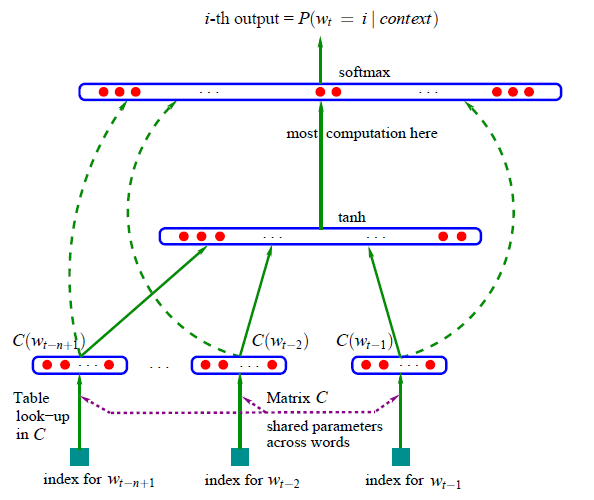
\includegraphics[width =.8\textwidth]{img/bengio.png}
%    \caption{The prediction-based Neural Language Model proposed by Bentio et al,. $C_{(i)}$ is the $i^{th}$ word embedding~\protect\cite{bengio2003neural}.}
%    \label{fig:Bengio}
%\end{figure}

These vectors are then fed to the hidden layer, and its output is passed on to the, so-called softmax layer, which predicts the next word of the sequence. A softmax layer is the final output layer of a neural network which performs classification calculations. The layer receives the output from the softmax function, which takes as an input a number of scores values from the previous layer and translates them into numbers in the range between 0 and 1, where the sum equals 1, resulting in a true representation of a probability distribution \cite{buduma2017fundamentals}. 
This method's problem lies within the size of the softmax layer, as the computing effort relies on the number of words in the vocabulary, which can be very high, leading to high computation costs.

\textbf{Word2vec Embeddings} 
\label{sec:Word2vec_embeddings}

A huge milestone were the so called Word2vec embedding models introduced by Mikolov et al. in 2013 \cite{mikolov2013efficient}. 
Word2vec models generate distributed word representations by using either continuous bag-of-words or the continuous skip-gram model architectures. 
Bag-of-words models take $n$-words before and $n$-words after the target word into consideration for their prediction. The word order does not influence the prediction. Mikolov et al. managed to efficiently improve the training by removing the hidden layer and approximating the objective. That way, they could improve training speed, accuracy and the efficiency of large-scale training of word embedding on huge amounts of text data.
Moreover, they found that the training on huge corpora enabled them to automatically capture relationships and similarities between words in text data, such as country - capital, or gender relationships, as shown in Figure~\ref{fig:Word2Vec}.

\begin{figure}
    \centering
    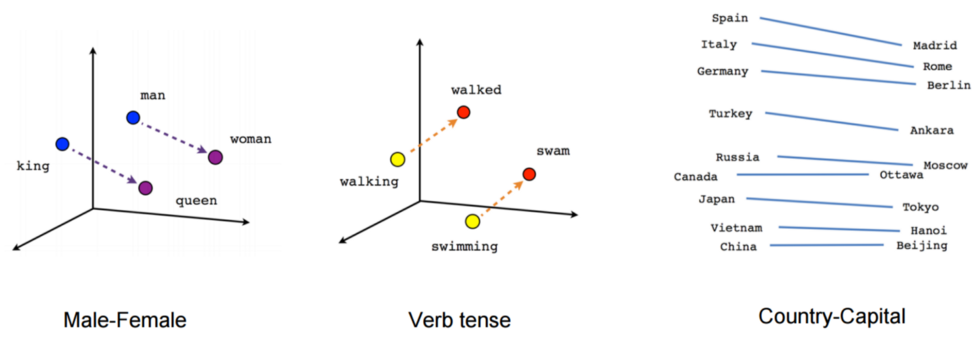
\includegraphics[ width = .8\textwidth]{img/Word2Vec_relations.png}
    \caption{Word2Vec representations capturing relationships and similarities between words, such as gender relationships, tenses and country-capital relations. Illustrated by~\protect\cite{Bujokas:2020}}
    \label{fig:Word2Vec}
\end{figure}


To summarize, the Word2vec is a shallow, two-layer neural network trained to generate a word embedding to represent linguistic contexts of words. It takes as an input a large text corpus and generates a vector space, consisting of several hundred dimensions, where each unique word in the corpus is assigned to a corresponding vector in the vector space. In the vector space, word vectors are positioned such that words that have common context in the corpus are located close to one another \cite{mikolov2013efficient}, as illustrated in Figure~\ref{fig:Word2Vec_bogdan}. The problem with Word2vec models is that they are not able to represent ambiguity of words.
For example, the word "Apple" has the same representation in "Apple Pie" and "Apple Computer". 

\begin{figure}
    \centering
    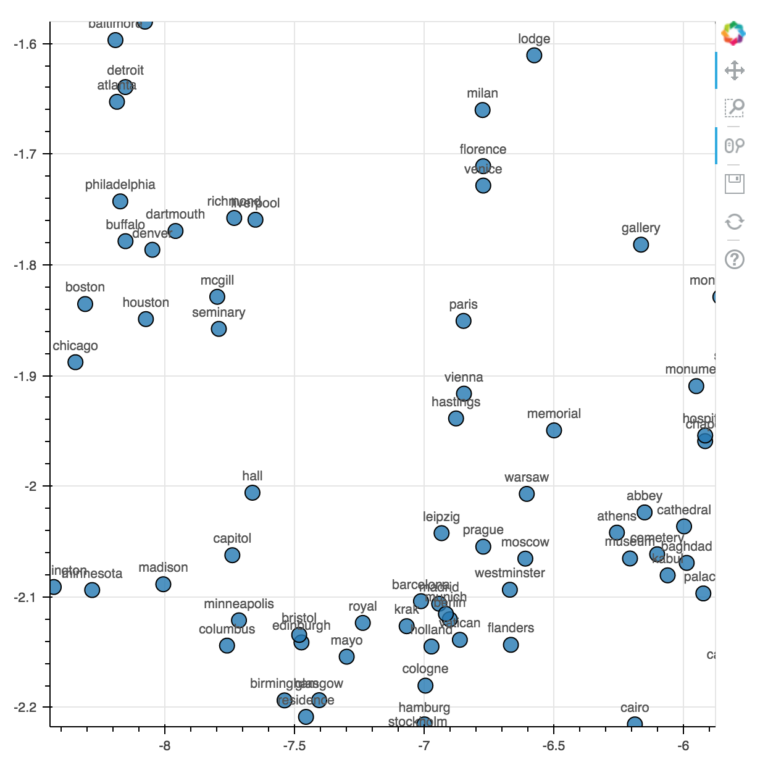
\includegraphics[ width = .7\textwidth]{img/Wod2Vec_representations_embedding.png}
    \caption{A 2D t-SNE visualisation of Word2Vec embedding representations.~\protect\cite{Bogdan:2018}}
    \label{fig:Word2Vec_bogdan}
\end{figure}

\textbf{Recurrent Neural Networks}
    \label{sec:RNNs}

Around 2014, Recurrent Neural Networks (RNN) were broadly adopted in the field of natural language processing \cite{jozefowicz2016exploring}.RNNs are so-called Sequene-to-Sequence models that transform sequences of data (e.g. text, audio, video) into sequences of another type. Examples for the usage of these transformations are translation or classification tasks.

In practice, RNNs have shown to have difficulties processing long sentences, since they handle sequences word by word in a sequential fashion. This makes them prone to loose memory of distant positions in the sequence \cite{mikolov2010recurrent}.
Due to their vanishing and exploding gradient problem \cite{pascanu2013difficulty}, the RNN architecture was extended by long-short term memory networks (LSTM) \cite{hochreiter1997long, graves2005framewise}. 
LSTM networks are similar to RNNs, with the difference that they can process whole data sequences, instead of only single data points, which allows for improved determination of the storage of long-range dependencies in data. 

Latest NLP systems aim for the full understanding of text, checking syntactic and semantic validity of linguistic input, using real-world knowledge, speech acts, conversation and discourse structures \cite{kumar2011natural}.
Full understanding of text largely depends on the context it appears in. 
Deep contextual word representations have shown that they are able to model complex characteristics of word usage (e.g. syntax and semantics), and the variety of word usage in different linguistic contexts (e.g. polysemy) \cite{peters2018deep}. They generate a vector representation of each word that is based on the context (or the other words in the sentence) it appears in - to capture the word meaning in that context as well as other additional contextual information. Deep contextual word representations, first introduced by Peters et al. rely on a bidirectional LSTM, trained with a coupled language model objective on a large text corpus and are, therefore, called ELMo (Embeddings from Language Models) representations.
Instead of using fixed embedding representations, like Word2vec or GloVe \cite{pennington2014glove} for each word, ELMo "looks" at the entire sentence before assigning it an embedding. 

\textbf{Attention Mechanism}
\label{sec:attention}
%Attention nochmal besser schreiben
\todo{Attention nochmal besser beschreiben}
In 2015 various papers described the concept of "attention" in training recurrent neural networks, allowing models to learn alignments between different modalities \cite{mnih2014recurrent, bahdanau2014neural}. These models use information form learning to decide which parts of the input to pay attention to in order to draw global dependencies between input and output. 

The models are based on an encoder-decoder structure, where the encoder maps the input sequence of character representations to a sequence of continuous representations. In the second step, the decoder creates an output, a sequence of characters. 

The attention in the decoder allows it to look back at the hidden state of the source sequences, which are combined using a weighted average and then serve as an additional input to the decoder. 
An advanced approach of attention is called self-attention, which allows for obtaining more contextually sensitive word representations by looking at nearby words in a sentence or paragraph. Google's machine translation team was the first in 2017 to use self-attention mechanisms in their paper "Attention is All You Need" to learn text representations \cite{vaswani2017attention}. To better understand self-attention one can imagine the human sight mechanism. While humans detect an object, say a banana, they will typically not scan the entire room, or scene to acquire information but rather focus on the respective object. Humans learn, that objects typically appear in a particular scene. E. g., bananas are typically in a fruit bowl. That way, they combine information from different fixations over time to build a representation and in the future, focus their attention on that particular scene, the bowl, when looking for the banana. 



\textbf{Transformer Models}
\label{sec:transformers}

In 2017 Vaswani et al. introduced the Transformer, a novel model architecture relying entirely on the attention mechanism \cite{vaswani2017attention}. They use stacked self-attention and point-wise, fully connected layers for en- and decoding. 
The self-attention based Transformer model is not recurrent, hence the output is not fed back as input like in RNNs but uses its attention to "look back" to the crucial piece of information. Text sequences are not memorized or stored completely but rather the parts, which are considered relevant. This approach allows the Transformer to outperform RNNs and LSTM networks and makes the model more parallelizable, resulting in enhanced computational performance. Transformer models proved to improve the state-of-the-art approaches in the field \cite{vaswani2017attention}. 

Famous Transformer models are ERNIE \cite{zhang2019ernie}, BERT \cite{devlin2018bert}, XLnet \cite{yang2019xlnet}, RoBERTa \cite{liu2019roberta}, and DistilBERT \cite{sanh2019distilbert}. More detailed information about the Transformer Model BERT is provided in chapter~\ref{sec:bert}.

\subsubsection{Tasks in NLP}
\label{sec:tasks_in_nLP}

Next to MT, there is a broad scope of tasks NLP is used for. Some prominent examples are speech recognition, language detection, part-of-speech tagging, sentiment analysis (SA), question answering, automatic summarization, text classification, character recognition, textual entailment, and many more.

NLP tasks can be divided in two main fields: analysis, and generation tasks. Analysis tasks aim for analysing existing text, while the objective of generation tasks is to generate new text. The analysis task can again be divided into syntactic, a language structure-based task, semantic, a meaning based task and pragmatic, a task of open difficult problems to solve \cite{ganegedara2018natural}. 
Figure ~\ref{fig:NLP-Tasks-Taxonomy} illustrates the categorization of different NLP task as described by Ganegadara. 
\begin{figure}
    \centering
    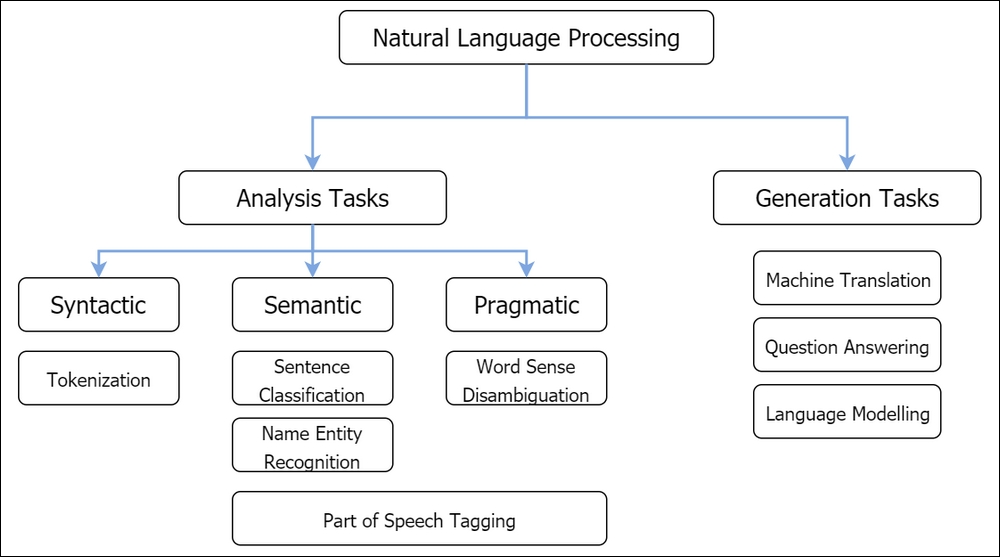
\includegraphics[ width = .7\textwidth]{img/NLP_tasks.jpg}
    \caption{A taxonomy of popular NLP tasks~\protect\cite{ganegedara2018natural}}
    \label{fig:NLP-Tasks-Taxonomy}
\end{figure}
Examples for semantic tasks are SA and Aspect-based Sentiment Analysis (ABSA). 
SA is an active field of research in NLP that aims to detect opinions in (mostly user-generated) text. The perceived sentiment, which occurs in user comments, feedback questionnaires, or critiques, provides valuable information for various purposes. Sentiment is usually expressed in either two categories: positive and negative, or on an $n$-point scale (e.g., very good, good, satisfactory, sufficient, insufficient). Thus, a sentiment analysis task can be interpreted as a classification task, where each class represents a sentiment \cite{prabowo2009sentiment}. Figure ~\ref{fig:SA} shows an example of the sentiment analysis task using a BERT language model, which will be described in section ~\ref{sec:bert}.

\begin{figure}
\centering

\tikzset{every picture/.style={line width=0.75pt}} %set default line width to 0.75pt

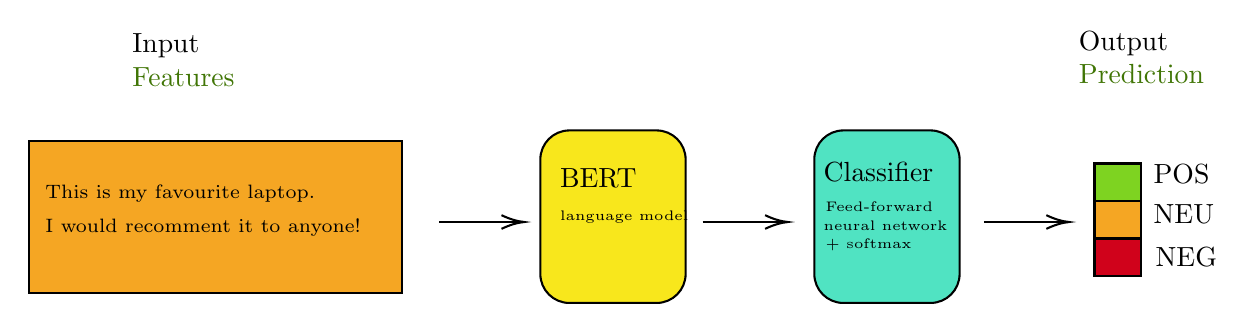
\begin{tikzpicture}[x=0.75pt,y=0.75pt,yscale=-1,xscale=1]
%uncomment if require: \path (0,218); %set diagram left start at 0, and has height of 218

%Shape: Rectangle [id:dp7006294352286838] 
\draw  [fill={rgb, 255:red, 245; green, 166; blue, 35 }  ,fill opacity=1 ] (14.5,104.13) -- (194.3,104.13) -- (194.3,177.13) -- (14.5,177.13) -- cycle ;
%Straight Lines [id:da6575723888982618] 
\draw    (212.23,143.13) -- (251.23,143.13) ;
\draw [shift={(253.23,143.13)}, rotate = 180] [color={rgb, 255:red, 0; green, 0; blue, 0 }  ][line width=0.75]    (10.93,-3.29) .. controls (6.95,-1.4) and (3.31,-0.3) .. (0,0) .. controls (3.31,0.3) and (6.95,1.4) .. (10.93,3.29)   ;
%Rounded Rect [id:dp8363863646203258] 
\draw  [fill={rgb, 255:red, 248; green, 231; blue, 28 }  ,fill opacity=1 ] (261,113) .. controls (261,105.27) and (267.27,99) .. (275,99) -- (317,99) .. controls (324.73,99) and (331,105.27) .. (331,113) -- (331,168.13) .. controls (331,175.87) and (324.73,182.13) .. (317,182.13) -- (275,182.13) .. controls (267.27,182.13) and (261,175.87) .. (261,168.13) -- cycle ;
%Straight Lines [id:da9521339561624853] 
\draw    (339.23,143.13) -- (378.23,143.13) ;
\draw [shift={(380.23,143.13)}, rotate = 180] [color={rgb, 255:red, 0; green, 0; blue, 0 }  ][line width=0.75]    (10.93,-3.29) .. controls (6.95,-1.4) and (3.31,-0.3) .. (0,0) .. controls (3.31,0.3) and (6.95,1.4) .. (10.93,3.29)   ;
%Rounded Rect [id:dp0334875358297424] 
\draw  [fill={rgb, 255:red, 80; green, 227; blue, 194 }  ,fill opacity=1 ] (393,113) .. controls (393,105.27) and (399.27,99) .. (407,99) -- (449,99) .. controls (456.73,99) and (463,105.27) .. (463,113) -- (463,168.13) .. controls (463,175.87) and (456.73,182.13) .. (449,182.13) -- (407,182.13) .. controls (399.27,182.13) and (393,175.87) .. (393,168.13) -- cycle ;
%Straight Lines [id:da2921180358184613] 
\draw    (474.73,143.13) -- (513.73,143.13) ;
\draw [shift={(515.73,143.13)}, rotate = 180] [color={rgb, 255:red, 0; green, 0; blue, 0 }  ][line width=0.75]    (10.93,-3.29) .. controls (6.95,-1.4) and (3.31,-0.3) .. (0,0) .. controls (3.31,0.3) and (6.95,1.4) .. (10.93,3.29)   ;
%Shape: Rectangle [id:dp439847396677838] 
\draw  [fill={rgb, 255:red, 126; green, 211; blue, 33 }  ,fill opacity=1 ] (528,114.93) -- (550.4,114.93) -- (550.4,133) -- (528,133) -- cycle ;
%Shape: Rectangle [id:dp6078072626477552] 
\draw  [fill={rgb, 255:red, 245; green, 166; blue, 35 }  ,fill opacity=1 ] (528,133) -- (550.4,133) -- (550.4,151.07) -- (528,151.07) -- cycle ;
%Shape: Rectangle [id:dp7563474548449828] 
\draw  [fill={rgb, 255:red, 208; green, 2; blue, 27 }  ,fill opacity=1 ] (528,151.07) -- (550.4,151.07) -- (550.4,169.13) -- (528,169.13) -- cycle ;

% Text Node
\draw (63,51) node [anchor=north west][inner sep=0.75pt]   [align=left] {Input\\\textcolor[rgb]{0.25,0.46,0.02}{Features}};
% Text Node
\draw (21,124) node [anchor=north west][inner sep=0.75pt]   [align=left] {{\scriptsize This is my favourite laptop. }\\{\scriptsize I would recomment it to anyone!}};
% Text Node
\draw (269,116) node [anchor=north west][inner sep=0.75pt]   [align=left] {BERT \\{\tiny language model}};
% Text Node
\draw (396,113) node [anchor=north west][inner sep=0.75pt]   [align=left] {Classifier};
% Text Node
\draw (555,114) node [anchor=north west][inner sep=0.75pt]   [align=left] {POS};
% Text Node
\draw (555,133) node [anchor=north west][inner sep=0.75pt]   [align=left] {NEU};
% Text Node
\draw (556,154) node [anchor=north west][inner sep=0.75pt]   [align=left] {NEG};
% Text Node
\draw (519,50) node [anchor=north west][inner sep=0.75pt]   [align=left] {Output\\\textcolor[rgb]{0.25,0.46,0.02}{Prediction}};
% Text Node
\draw (397,132) node [anchor=north west][inner sep=0.75pt]   [align=left] {{\tiny Feed-forward }};
% Text Node
\draw (396,141) node [anchor=north west][inner sep=0.75pt]   [align=left] {{\tiny neural network }};
% Text Node
\draw (397,150) node [anchor=north west][inner sep=0.75pt]   [align=left] {{\tiny + softmax}};

\end{tikzpicture}
    \caption{Sentiment Analysis of Laptop Reviews}
    \label{fig:SA}
\end{figure}


In contrast to SA, ABSA is a more fine-grained task, which consists of two main subtasks, namely Aspect-Category Detection, and Aspect-Category Sentiment Classification. In the first (multi-label classification \footnote{in single-label classification one sample in the data contains exactly one output label, while in the multi-label classification task, one sample can contain n output labels.}) task, a sentence is associated with a set of predefined single- and multi-word aspect terms (e.g., "operation performance", "battery"). The second task, the Aspect-Category Sentiment Classification, deals with the detection of sentiment associated with its aspect (e.g. "positive", "neutral", "negative") \cite{pavlopoulos2014aspect}. See Figure ~\ref{fig:ABSA} for an illustration of the ABSA task.


\begin{figure}
\centering

\tikzset{every picture/.style={line width=0.75pt}} %set default line width to 0.75pt

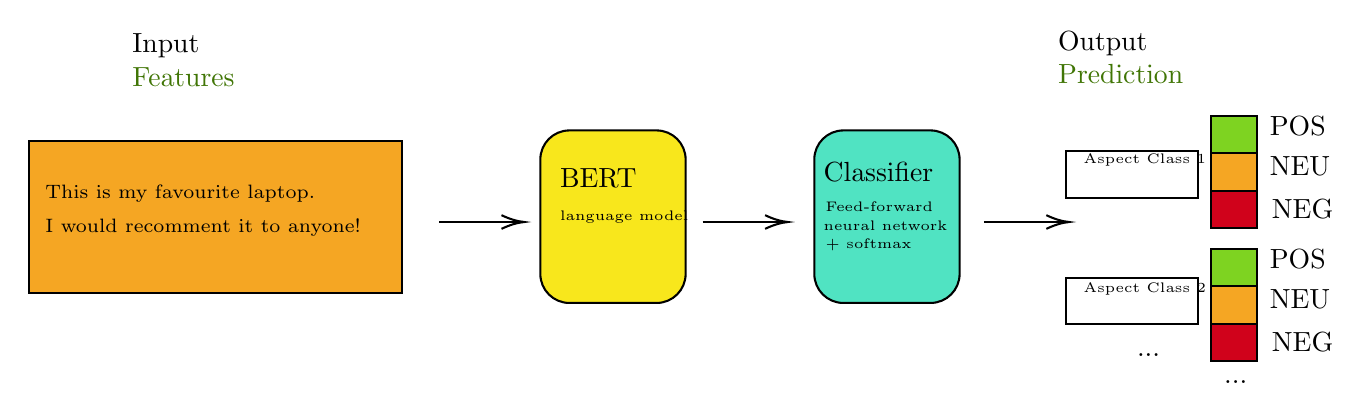
\begin{tikzpicture}[x=0.75pt,y=0.75pt,yscale=-1,xscale=1]
%uncomment if require: \path (0,341); %set diagram left start at 0, and has height of 341

%Shape: Rectangle [id:dp7006294352286838] 
\draw  [fill={rgb, 255:red, 245; green, 166; blue, 35 }  ,fill opacity=1 ] (14.5,104.13) -- (194.3,104.13) -- (194.3,177.13) -- (14.5,177.13) -- cycle ;
%Straight Lines [id:da6575723888982618] 
\draw    (212.23,143.13) -- (251.23,143.13) ;
\draw [shift={(253.23,143.13)}, rotate = 180] [color={rgb, 255:red, 0; green, 0; blue, 0 }  ][line width=0.75]    (10.93,-3.29) .. controls (6.95,-1.4) and (3.31,-0.3) .. (0,0) .. controls (3.31,0.3) and (6.95,1.4) .. (10.93,3.29)   ;
%Rounded Rect [id:dp8363863646203258] 
\draw  [fill={rgb, 255:red, 248; green, 231; blue, 28 }  ,fill opacity=1 ] (261,113) .. controls (261,105.27) and (267.27,99) .. (275,99) -- (317,99) .. controls (324.73,99) and (331,105.27) .. (331,113) -- (331,168.13) .. controls (331,175.87) and (324.73,182.13) .. (317,182.13) -- (275,182.13) .. controls (267.27,182.13) and (261,175.87) .. (261,168.13) -- cycle ;
%Straight Lines [id:da9521339561624853] 
\draw    (339.23,143.13) -- (378.23,143.13) ;
\draw [shift={(380.23,143.13)}, rotate = 180] [color={rgb, 255:red, 0; green, 0; blue, 0 }  ][line width=0.75]    (10.93,-3.29) .. controls (6.95,-1.4) and (3.31,-0.3) .. (0,0) .. controls (3.31,0.3) and (6.95,1.4) .. (10.93,3.29)   ;
%Rounded Rect [id:dp0334875358297424] 
\draw  [fill={rgb, 255:red, 80; green, 227; blue, 194 }  ,fill opacity=1 ] (393,113) .. controls (393,105.27) and (399.27,99) .. (407,99) -- (449,99) .. controls (456.73,99) and (463,105.27) .. (463,113) -- (463,168.13) .. controls (463,175.87) and (456.73,182.13) .. (449,182.13) -- (407,182.13) .. controls (399.27,182.13) and (393,175.87) .. (393,168.13) -- cycle ;
%Straight Lines [id:da2921180358184613] 
\draw    (474.73,143.13) -- (513.73,143.13) ;
\draw [shift={(515.73,143.13)}, rotate = 180] [color={rgb, 255:red, 0; green, 0; blue, 0 }  ][line width=0.75]    (10.93,-3.29) .. controls (6.95,-1.4) and (3.31,-0.3) .. (0,0) .. controls (3.31,0.3) and (6.95,1.4) .. (10.93,3.29)   ;
%Shape: Rectangle [id:dp439847396677838] 
\draw  [fill={rgb, 255:red, 126; green, 211; blue, 33 }  ,fill opacity=1 ] (584,91.93) -- (606.4,91.93) -- (606.4,110) -- (584,110) -- cycle ;
%Shape: Rectangle [id:dp6078072626477552] 
\draw  [fill={rgb, 255:red, 245; green, 166; blue, 35 }  ,fill opacity=1 ] (584,110) -- (606.4,110) -- (606.4,128.07) -- (584,128.07) -- cycle ;
%Shape: Rectangle [id:dp7563474548449828] 
\draw  [fill={rgb, 255:red, 208; green, 2; blue, 27 }  ,fill opacity=1 ] (584,128.07) -- (606.4,128.07) -- (606.4,146.13) -- (584,146.13) -- cycle ;
%Shape: Rectangle [id:dp25079314597811353] 
\draw  [fill={rgb, 255:red, 126; green, 211; blue, 33 }  ,fill opacity=1 ] (584,155.93) -- (606.4,155.93) -- (606.4,174) -- (584,174) -- cycle ;
%Shape: Rectangle [id:dp724072679501146] 
\draw  [fill={rgb, 255:red, 245; green, 166; blue, 35 }  ,fill opacity=1 ] (584,174) -- (606.4,174) -- (606.4,192.07) -- (584,192.07) -- cycle ;
%Shape: Rectangle [id:dp120836736470876] 
\draw  [fill={rgb, 255:red, 208; green, 2; blue, 27 }  ,fill opacity=1 ] (584,192.07) -- (606.4,192.07) -- (606.4,210.13) -- (584,210.13) -- cycle ;
%Shape: Rectangle [id:dp6243646913162751] 
\draw   (514.3,109) -- (578,109) -- (578,131.47) -- (514.3,131.47) -- cycle ;
%Shape: Rectangle [id:dp06781285859521458] 
\draw   (514.3,170) -- (578,170) -- (578,192.47) -- (514.3,192.47) -- cycle ;

% Text Node
\draw (63,51) node [anchor=north west][inner sep=0.75pt]   [align=left] {Input\\\textcolor[rgb]{0.25,0.46,0.02}{Features}};
% Text Node
\draw (21,124) node [anchor=north west][inner sep=0.75pt]   [align=left] {{\scriptsize This is my favourite laptop. }\\{\scriptsize I would recomment it to anyone!}};
% Text Node
\draw (269,116) node [anchor=north west][inner sep=0.75pt]   [align=left] {BERT \\{\tiny language model}};
% Text Node
\draw (396,113) node [anchor=north west][inner sep=0.75pt]   [align=left] {Classifier};
% Text Node
\draw (611,91) node [anchor=north west][inner sep=0.75pt]   [align=left] {POS};
% Text Node
\draw (611,110) node [anchor=north west][inner sep=0.75pt]   [align=left] {NEU};
% Text Node
\draw (612,131) node [anchor=north west][inner sep=0.75pt]   [align=left] {NEG};
% Text Node
\draw (509,50) node [anchor=north west][inner sep=0.75pt]   [align=left] {Output\\\textcolor[rgb]{0.25,0.46,0.02}{Prediction}};
% Text Node
\draw (397,132) node [anchor=north west][inner sep=0.75pt]   [align=left] {{\tiny Feed-forward }};
% Text Node
\draw (396,141) node [anchor=north west][inner sep=0.75pt]   [align=left] {{\tiny neural network }};
% Text Node
\draw (397,150) node [anchor=north west][inner sep=0.75pt]   [align=left] {{\tiny + softmax}};
% Text Node
\draw (611,155) node [anchor=north west][inner sep=0.75pt]   [align=left] {POS};
% Text Node
\draw (611,174) node [anchor=north west][inner sep=0.75pt]   [align=left] {NEU};
% Text Node
\draw (612,195) node [anchor=north west][inner sep=0.75pt]   [align=left] {NEG};
% Text Node
\draw (589,218) node [anchor=north west][inner sep=0.75pt]   [align=left] {...};
% Text Node
\draw (547,205) node [anchor=north west][inner sep=0.75pt]   [align=left] {...};
% Text Node
\draw (521.3,109) node [anchor=north west][inner sep=0.75pt]   [align=left] {{\tiny Aspect Class 1}};
% Text Node
\draw (521.3,171) node [anchor=north west][inner sep=0.75pt]   [align=left] {{\tiny Aspect Class 2}};


\end{tikzpicture}
    \caption{Aspect Based Sentiment Analysis of Laptop Reviews}
    \label{fig:ABSA}
\end{figure}



%-------------------------------------------------------------------
%----------------------------BERT-----------------------------------
%------------------------------------------------------------------


\subsection{Bidirectional Encoder Representations from Transformers}
\label{sec:bert}
In 2018, Google AI researchers achieved a breakthrough in NLP by introducing BERT, a deep contextual language representation model. BERT is an abbreviation for Bidirectional Encoder Representations from Transformers \cite{devlin2018bert}. It is built on preceding innovations: deep contextualized word representations \cite{peters2018deep}, the Transformer architecture \cite{vaswani2017attention}, and pre-training on a language modeling task with subsequent fine-tuning on a downstream task \cite{radford2018improving, howard2018universal}.

\begin{figure}
    \centering
    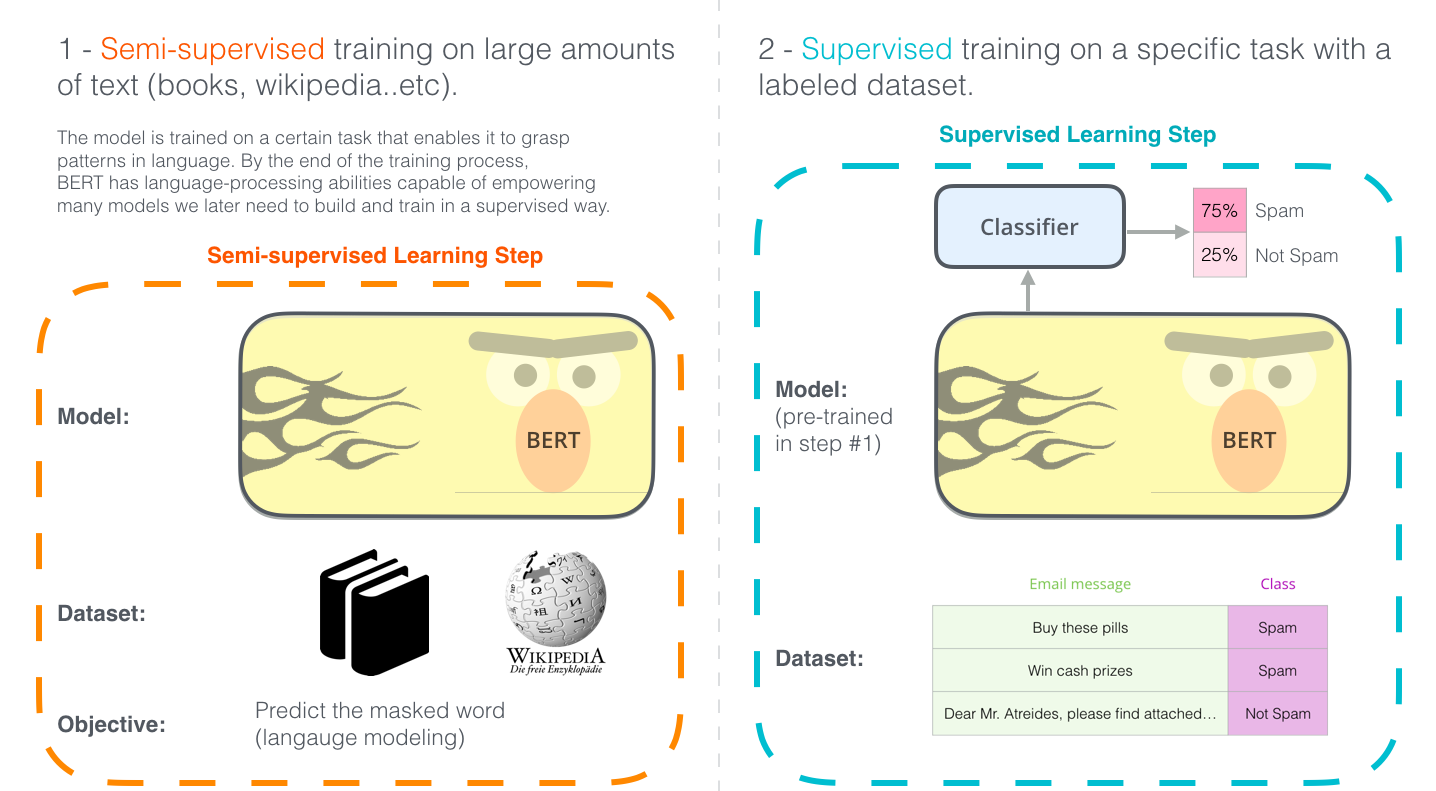
\includegraphics[ width = .8\textwidth]{img/bert-pre-training_fine-tuning.png}
    \caption{The BERT workflow consists of (1) pre-training: self-supervised training on a large amount of text (books and Wikipedia) and (2) fine-tuning: supervised training on a downstream task with labeled data. Illustration from~\protect\cite{alammar2018illustrated}.}
    \label{fig:BERT}
\end{figure}


\subsubsection{Model Architecture}
\label{sec:bert_architecture}
% elaborate
BERT is a stack of transformer encoder layers that consist of a multi-head attention layer (heads), followed by a fully-connected neural networks.
For every input token in a text sequence,( e.g., a sentence), each head computes key, value, and query vectors, which are then used to create a weighted representation. The outputs of all heads in the same layer are combined and run through a fully-connected layer.

BERT uses the self-attention mechanism introduced with the Transformer model \cite{vaswani2017attention} and described in chapter~\ref{sec:attention}. 
%Fig xy exposes an example of how BERT uses the self-attention mechanism....


Similar to the Word2vec word embedding, BERT does map related words closely, but it is context-sensitive, meaning a different word vector is computed for a word if encountered in different contexts. In other terms, related words have a smaller distance in the word embedding than unrelated words, but can be discriminated by their context as BERT makes use of the information of the tokens in the sequence surrounding the word of interest.

To compute the input-encoding, BERT first tokenizes the given sentences into referring word pieces and then combines three input embedding layers (token, position, and segment) to obtain a fixed-length vector per token. Figure ~\ref{fig:BERT_Layers} gives an overview of the embedding layer architecture.

\textbf{Vocabulary Generation}

An important part of producing word embeddings is tokenization. As stated before, a word embedding is a feature vector representation of a word. A feature vector is a list of values generated to represent one word, where the values are floating points and can be positive and negative. The distance of word embeddings displays the distance of word similarity. To give an example, the word embedding for the word "cat" could be

\texttt{<0.4125, -1.6098, 0.6047, ..., -1.4257, -1.231>}.


BERT has a fixed set of learned word embeddings, composed in a word embedding lookup-table. Every row in this table corresponds to one word, and every column represents a feature of one token.
BERT large has a vocabulary of 30,522 tokens and 786 features in its embedding. For simplicity, Figure ~\ref{fig:word_embedding} shows a table of only 10 words tokens and 5 features.

\begin{figure}
\centering

\tikzset{every picture/.style={line width=0.75pt}} %set default line width to 0.75pt

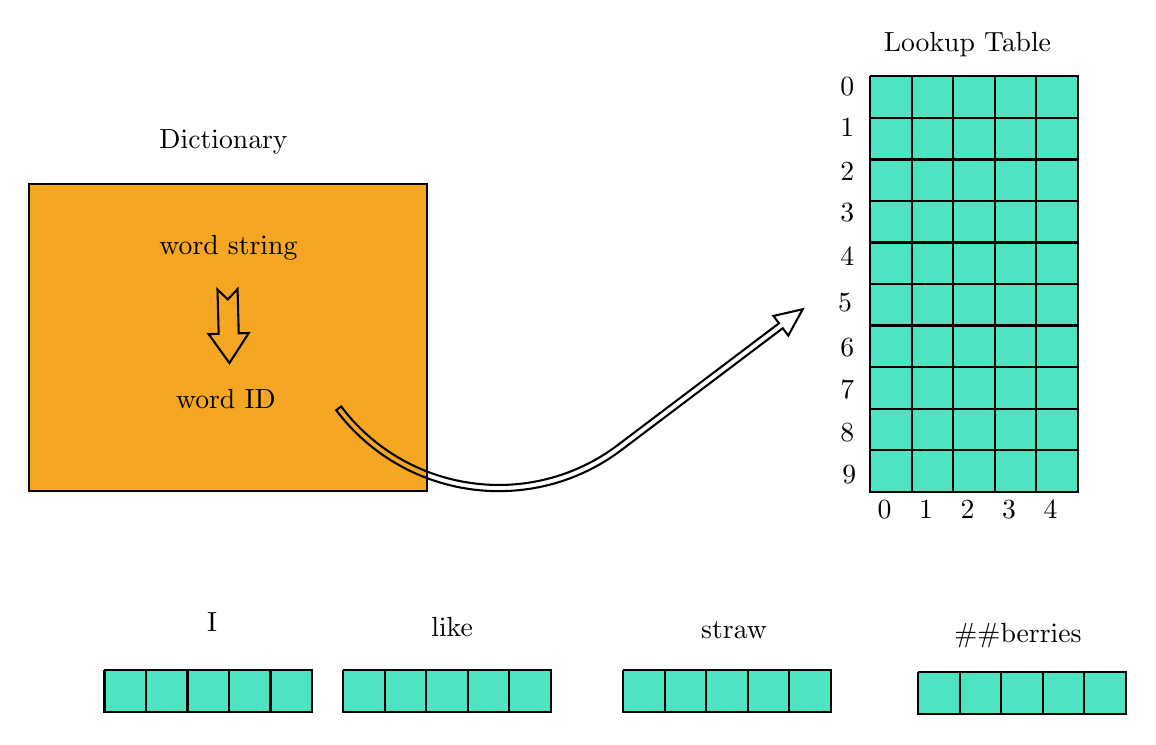
\begin{tikzpicture}[x=0.75pt,y=0.75pt,yscale=-1,xscale=1]
%uncomment if require: \path (0,412); %set diagram left start at 0, and has height of 412

%Shape: Rectangle [id:dp7006294352286838] 
\draw  [fill={rgb, 255:red, 245; green, 166; blue, 35 }  ,fill opacity=1 ] (42.5,97.65) -- (234.5,97.65) -- (234.5,245.65) -- (42.5,245.65) -- cycle ;
%Notched Right Arrow [id:dp3093746656409001] 
\draw   (143.13,148.46) -- (143.68,169.75) -- (148.51,169.63) -- (139.21,184.07) -- (129.17,170.12) -- (134.01,170) -- (133.46,148.7) -- (138.42,153.42) -- cycle ;
%Shape: Grid [id:dp4237249967627763] 
\draw  [draw opacity=0][fill={rgb, 255:red, 80; green, 227; blue, 194 }  ,fill opacity=1 ] (448,46) -- (548.45,46) -- (548.45,246.48) -- (448,246.48) -- cycle ; \draw   (448,46) -- (448,246.48)(468,46) -- (468,246.48)(488,46) -- (488,246.48)(508,46) -- (508,246.48)(528,46) -- (528,246.48)(548,46) -- (548,246.48) ; \draw   (448,46) -- (548.45,46)(448,66) -- (548.45,66)(448,86) -- (548.45,86)(448,106) -- (548.45,106)(448,126) -- (548.45,126)(448,146) -- (548.45,146)(448,166) -- (548.45,166)(448,186) -- (548.45,186)(448,206) -- (548.45,206)(448,226) -- (548.45,226)(448,246) -- (548.45,246) ; \draw    ;
%Bend Arrow [id:dp1033529280692509] 
\draw   (190.67,206.82) -- (190.67,206.82) .. controls (223.32,250.05) and (284.84,258.63) .. (328.08,225.98) -- (405.77,167.31) -- (408.45,170.85) -- (415.43,158.15) -- (401.3,161.38) -- (403.98,164.93) -- (326.28,223.6) .. controls (284.36,255.26) and (224.71,246.94) .. (193.04,205.02) -- (193.04,205.02) -- cycle ;
%Shape: Grid [id:dp17330989415915177] 
\draw  [draw opacity=0][fill={rgb, 255:red, 80; green, 227; blue, 194 }  ,fill opacity=1 ] (79,332) -- (179.67,332) -- (179.67,352.82) -- (79,352.82) -- cycle ; \draw   (79,332) -- (79,352.82)(99,332) -- (99,352.82)(119,332) -- (119,352.82)(139,332) -- (139,352.82)(159,332) -- (159,352.82)(179,332) -- (179,352.82) ; \draw   (79,332) -- (179.67,332)(79,352) -- (179.67,352) ; \draw    ;
%Shape: Grid [id:dp2416280342144621] 
\draw  [draw opacity=0][fill={rgb, 255:red, 80; green, 227; blue, 194 }  ,fill opacity=1 ] (194,332) -- (294.67,332) -- (294.67,352.82) -- (194,352.82) -- cycle ; \draw   (194,332) -- (194,352.82)(214,332) -- (214,352.82)(234,332) -- (234,352.82)(254,332) -- (254,352.82)(274,332) -- (274,352.82)(294,332) -- (294,352.82) ; \draw   (194,332) -- (294.67,332)(194,352) -- (294.67,352) ; \draw    ;
%Shape: Grid [id:dp9264270742131507] 
\draw  [draw opacity=0][fill={rgb, 255:red, 80; green, 227; blue, 194 }  ,fill opacity=1 ] (329,332) -- (429.67,332) -- (429.67,352.82) -- (329,352.82) -- cycle ; \draw   (329,332) -- (329,352.82)(349,332) -- (349,352.82)(369,332) -- (369,352.82)(389,332) -- (389,352.82)(409,332) -- (409,352.82)(429,332) -- (429,352.82) ; \draw   (329,332) -- (429.67,332)(329,352) -- (429.67,352) ; \draw    ;
%Shape: Grid [id:dp20800430109446355] 
\draw  [draw opacity=0][fill={rgb, 255:red, 80; green, 227; blue, 194 }  ,fill opacity=1 ] (471,333) -- (571.67,333) -- (571.67,353.82) -- (471,353.82) -- cycle ; \draw   (471,333) -- (471,353.82)(491,333) -- (491,353.82)(511,333) -- (511,353.82)(531,333) -- (531,353.82)(551,333) -- (551,353.82)(571,333) -- (571,353.82) ; \draw   (471,333) -- (571.67,333)(471,353) -- (571.67,353) ; \draw    ;

% Text Node
\draw (104,70) node [anchor=north west][inner sep=0.75pt]   [align=left] {Dictionary};
% Text Node
\draw (104,121) node [anchor=north west][inner sep=0.75pt]   [align=left] {word string};
% Text Node
\draw (112,195) node [anchor=north west][inner sep=0.75pt]   [align=left] {word ID};
% Text Node
\draw (453,23) node [anchor=north west][inner sep=0.75pt]   [align=left] {Lookup Table};
% Text Node
\draw (432,45) node [anchor=north west][inner sep=0.75pt]   [align=left] {0};
% Text Node
\draw (127,303) node [anchor=north west][inner sep=0.75pt]   [align=left] {I};
% Text Node
\draw (450,249) node [anchor=north west][inner sep=0.75pt]   [align=left] {0 \ \ 1 \ \ 2 \ \ 3 \ \ 4 };
% Text Node
\draw (235,305) node [anchor=north west][inner sep=0.75pt]   [align=left] {like};
% Text Node
\draw (365,307) node [anchor=north west][inner sep=0.75pt]   [align=left] {straw};
% Text Node
\draw (487,308) node [anchor=north west][inner sep=0.75pt]   [align=left] {\#\#berries};
% Text Node
\draw (432,65) node [anchor=north west][inner sep=0.75pt]   [align=left] {1};
% Text Node
\draw (432,86) node [anchor=north west][inner sep=0.75pt]   [align=left] {2};
% Text Node
\draw (432,106) node [anchor=north west][inner sep=0.75pt]   [align=left] {3};
% Text Node
\draw (432,127) node [anchor=north west][inner sep=0.75pt]   [align=left] {4};
% Text Node
\draw (431,149) node [anchor=north west][inner sep=0.75pt]   [align=left] {5};
% Text Node
\draw (432,171) node [anchor=north west][inner sep=0.75pt]   [align=left] {6};
% Text Node
\draw (432,191) node [anchor=north west][inner sep=0.75pt]   [align=left] {7};
% Text Node
\draw (432,212) node [anchor=north west][inner sep=0.75pt]   [align=left] {8};
% Text Node
\draw (433,232) node [anchor=north west][inner sep=0.75pt]   [align=left] {9};


\end{tikzpicture}
\caption{The conversion of a sequence string into its word vector representations.}
    \label{fig:word_embedding}

\end{figure}

A dictionary converts a word string into the corresponding word-id in the word embedding lookup table. 
When feeding a sequence of words into the BERT architecture, it will fist look up the word-ids in the dictionary and then take the corresponding word embeddings to get a sequence of word embeddings.
The Second Edition of the 20th volume Oxford English Dictionary contains entries for 171,476 words \cite{dictionary1989oxford}. In order to keep the size of the vocabulary as small as possible, not all words are included in the vocabulary. A WordPiece model breaks down unknown words into subwords \cite{wu2016google}. Given the word $embedding$. There is no representation for this word in the dictionary. The WordPiece method breaks the word down into the three word pieces $em$, $\#\#bed$, and $\#\#ding$, which are entries in the dictionary. That way the sequence, the word "embedding" appears in, consists of two additional tokens. Except for the first token, subwords are marked with two hash-symbols in front of the characters. Therefore, the subword $bed$ in the word $bedding$ does not have the same vector representation as the one in the word $embedding$ since it is the first token of the word and does not contain the two hash symbols. The WordPiece representation for the word $bedding$ is $bed$, $\#\#ding$, which conveys the information, that the word $bedding$ is related to the word $bed$.
The words stored in the dictionary differs, depending on the corpus, used for vocabulary generation.

\begin{figure}
    \centering
    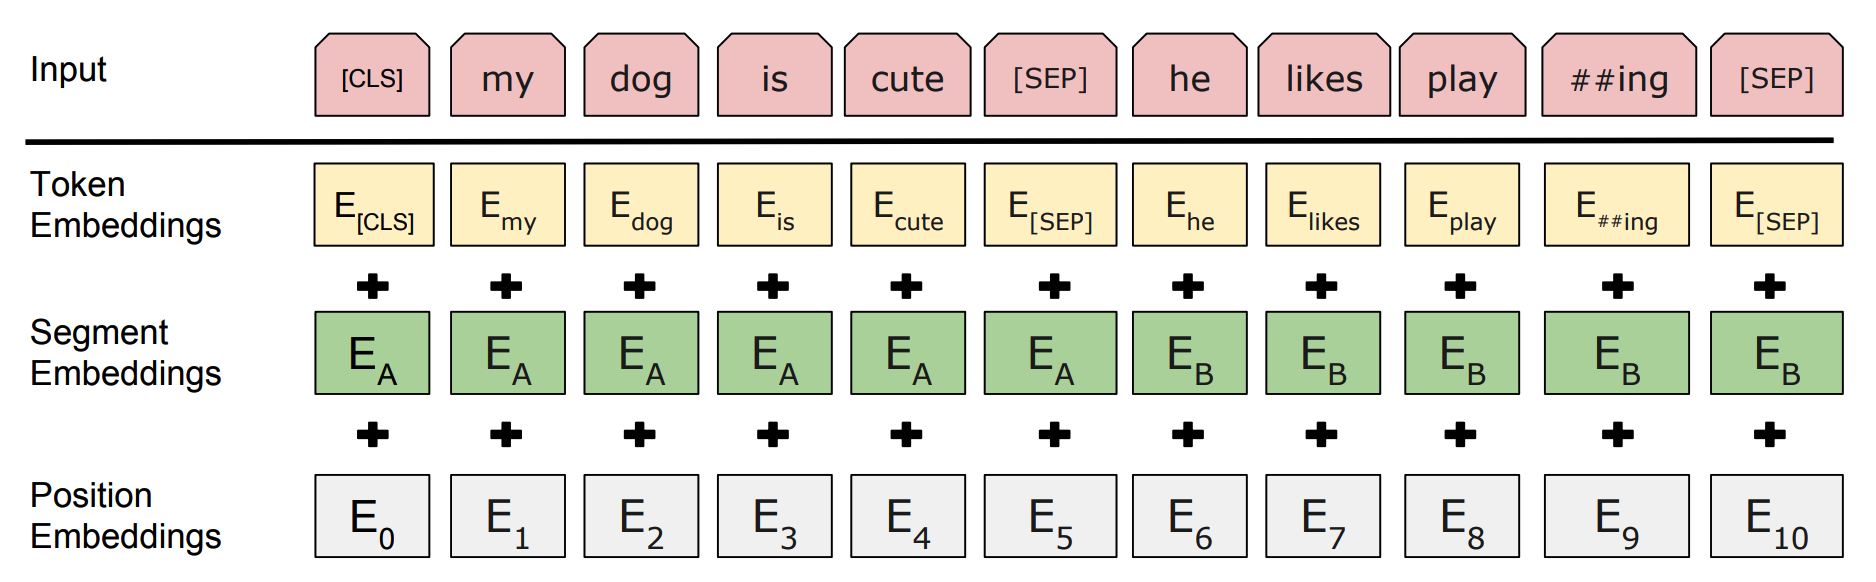
\includegraphics[ width = 1\textwidth]{img/bert_input_representatino.png}
    \caption{Three BERT embedding layers architecture: token, sequence, and positional embedding layers~\protect\cite{devlin2018bert}.}
    \label{fig:BERT_Layers}
\end{figure}
%----------------Token Embedding Layer------------------------------



\textbf{Token Embedding Layer}

The purpose of the token embedding layer is to transform the tokenized input (e.g. "I like strawberries") into a vector representation of fixed dimensions, as shown in Figure ~\ref{fig:BERT_tokenEmbedding}. In case of BERT base, each word is represented as a 768-dimensional vector.

\begin{figure}
\centering
    \begin{tikzpicture}[replace stretch/.style args={from #1 to #2 by #3}{%
        /utils/exec=\pgfmathsetmacro{\offlen}{#2-#1},
        dash pattern=on #1 off \offlen pt on 10cm,
        postaction={#3,dash pattern=on 0pt off #1 on \offlen pt off 10cm}}]
        
        % nodes
        \node[align=center] (start) [] {{\Large "I like strawberries"}\\\textit{3 words}};
        \node[align=center] (tokenized) [below of=start, yshift=-2cm] {{\Large"[CLS]", "I", "like", "straw", "\#\#berries", "[SEP]"}\\\textit{6 tokens}};
        \node (vectorized) [below of=tokenized, yshift=-2cm, draw, thick, minimum height=1.5cm, minimum width=3.5cm] {Token Embeddings};
        \draw [decorate,decoration={brace,amplitude=7pt, mirror}, asymbrace=0.75]
        (vectorized.south west) -- (vectorized.south east) node (vectorized_south)[black,midway,xshift=0.9cm, yshift=-0.5cm] {$768$};
        \draw [decorate,decoration={brace,amplitude=7pt}]
        (vectorized.north east) -- (vectorized.south east) node (vectorized_east)[black,midway,xshift=0.9cm, xshift=0.1cm, align=center]
        {$30.522$\\"words"};
        
        % tokenized object
        \node (0) [below of=vectorized, xshift=-5.5cm, yshift=-4.5cm, draw, thick, minimum height=1cm, minimum width=1.5cm] {\small [CLS]};
        \node (1) [right of=0, draw, xshift=0.5cm, thick, minimum height=1cm, minimum width=1.5cm] {\small I};
        \node (2) [right of=1, draw, xshift=0.5cm, thick, minimum height=1cm, minimum width=1.5cm] {\small love};
        \node (3) [right of=2, draw, xshift=0.5cm, thick, minimum height=1cm, minimum width=1.5cm] {\small straw};
        \node (4) [right of=3, draw, xshift=0.5cm, thick, minimum height=1cm, minimum width=1.5cm] {\small \#\#berries};
        \node (5) [right of=4, draw, xshift=0.5cm, thick, minimum height=1cm, minimum width=1.5cm] {\small [SEP]};
    
        \draw[thick,leaveout] (0.north west) -- ++(3,3);
        \draw[thick,leaveout] (1.north west) -- ++(3,3);
        \draw[thick,leaveout] (2.north west) -- ++(3,3);
        \draw[thick,leaveout] (3.north west) -- ++(3,3);
        \draw[thick,leaveout] (4.north west) -- ++(3,3);
        \draw[thick,leaveout] (5.north west) -- ++(3,3);
        \draw[thick,leaveout] (5.north east) -- ++(3,3);
        \draw[thick, replace stretch={from 2.16cm to 2.82cm by {-,draw=none}}] (5.south east) -- ++(3.03,3.03);
        
        \draw[thick] ([xshift=0.5cm, yshift=0.5cm] 0.north west) -- ++(9.05,0) -- ++(0,-1);
        \draw[thick] ([xshift=1cm, yshift=1cm] 0.north west) -- ++(9.05,0) -- ++(0,-1);
        \draw[thick] ([xshift=1.5cm, yshift=1.5cm] 0.north west) -- ++(9.05,0) -- ++(0,-1);
        \draw[thick] ([xshift=2cm, yshift=2cm] 0.north west) -- ++(9.05,0) -- ++(0,-1);
        \draw[thick] ([xshift=2.5cm, yshift=2.5cm] 0.north west) -- ++(9.05,0) -- ++(0,-1);
        \draw[thick] ([xshift=3cm, yshift=3cm] 0.north west) -- ++(9.05,0) -- ++(0,-1);
        
        \draw[thick] ([xshift=2cm, yshift=2cm] 0.north west) -- ++(0,-0.5);
        \draw[thick] ([xshift=2cm, yshift=2cm] 1.north west) -- ++(0,-0.5);
        \draw[thick] ([xshift=2cm, yshift=2cm] 2.north west) -- ++(0,-0.5);
        \draw[thick] ([xshift=2cm, yshift=2cm] 3.north west) -- ++(0,-0.5);
        \draw[thick] ([xshift=2cm, yshift=2cm] 4.north west) -- ++(0,-0.5);
        \draw[thick] ([xshift=2cm, yshift=2cm] 5.north west) -- ++(0,-0.5);
        \draw[thick] ([xshift=2cm, yshift=2cm] 5.south east) -- ++(-0.49,0);
        
        \draw [decorate,decoration={brace,amplitude=7pt, mirror}]
        (0.south west) -- (5.south east) node (vectorized_south)[black,midway,xshift=0cm, yshift=-0.5cm] {$6$};
        \draw [decorate,decoration={brace,amplitude=7pt, mirror}]
        (5.south east) -- ++(3,3) node (vectorized_south)[black,midway,xshift=0.4cm, yshift=-0.4cm] {\begin{turn}{45}$768$\end{turn}};
        \node at ([xshift=1.75cm, yshift=1.75cm] 5.south east) {\begin{turn}{45}\dots\end{turn}};
                
        % arrows
        \draw[->,thick] (start) -- node[right] () {\textbf{tokenization}} (tokenized.north);
        \draw[->,thick] (tokenized) -- node[right] () {\textbf{vector representation}} (vectorized.north);
        \draw[->,thick] (vectorized) -- ++(0,-2cm);

    \end{tikzpicture}
\caption{BERTbase Token Embedding Layer.} 
\label{fig:BERT_tokenEmbedding}
\end{figure}

Special tokens are needed for sentence classification. $"[CLS]"$ is added in front of every input example, and $"[SEP]"$ serves as a separator token.
As mentioned before, the tokenization method WordPiece, is used, which in this case splits the word "strawberries" into "straw" and "\#\#berries". 

%--------------Segment Embedding Layer------------------------------
\textbf{Segment Embedding Layer}

The purpose of the segment embedding layer is to enable BERT to distinguish inputs of a given sentence pair. Sentence pairs are used for example for the task of question answering, where text of interest and the question are differentiated like in "[CLS] He likes strawberries [SEP] What does he like?"
The segment embedding layer uses two indices 0 and 1 as vector representations to assign tokens to their corresponding input segment, see Figure \ref{fig:BERT_segmentEmbedding}.

\begin{figure}
\centering
\begin{tikzpicture}[replace stretch/.style args={from #1 to #2 by #3}{%
        /utils/exec=\pgfmathsetmacro{\offlen}{#2-#1},
        dash pattern=on #1 off \offlen pt on 10cm,
        postaction={#3,dash pattern=on 0pt off #1 on \offlen pt off 10cm}}]
        
        % nodes
        \node[align=center] (start) [] {{\Large "I like strawberries"} \\ {\Large "I like ice cream"}\\\textit{2 inputs}};
        \node[align=center] (tokenized) [below of=start, yshift=-2cm] {{\Large"[CLS]", "I", "like", "straw", "\#\#berries", "[SEP]", "I", "like" "ice" "cream"}\\\textit{10 tokens}};
        \node (vectorized) [below of=tokenized, yshift=-2cm, draw, thick, minimum height=1.5cm, minimum width=3.5cm] {Segment Embeddings};
        \draw [decorate,decoration={brace,amplitude=7pt, mirror}, asymbrace=0.75]
        (vectorized.south west) -- (vectorized.south east) node (vectorized_south)[black,midway,xshift=0.9cm, yshift=-0.5cm] {$768$};
        \draw [decorate,decoration={brace,amplitude=7pt}]
        (vectorized.north east) -- (vectorized.south east) node (vectorized_east)[black,midway,xshift=0.4cm, xshift=0.1cm, align=center]
        {$2$};
        
        % tokenized object
        \node (0) [below of=vectorized, xshift=-6.5cm, yshift=-4.5cm, draw, thick, minimum height=1cm, minimum width=1cm] {\small 0};
        \node (1) [right of=0, draw, thick, minimum height=1cm, minimum width=1cm] {\small 0};
        \node (2) [right of=1, draw, thick, minimum height=1cm, minimum width=1cm] {\small 0};
        \node (3) [right of=2, draw, thick, minimum height=1cm, minimum width=1cm] {\small 0};
        \node (4) [right of=3, draw, thick, minimum height=1cm, minimum width=1cm] {\small 0};
        \node (5) [right of=4, draw, thick, minimum height=1cm, minimum width=1cm] {\small 0};
        \node (6) [right of=5, draw, thick, minimum height=1cm, minimum width=1cm] {\small 1};
        \node (7) [right of=6, draw, thick, minimum height=1cm, minimum width=1cm] {\small 1};
        \node (8) [right of=7, draw, thick, minimum height=1cm, minimum width=1cm] {\small 1};
        \node (9) [right of=8, draw, thick, minimum height=1cm, minimum width=1cm] {\small 1};
    
        \draw[thick,leaveout] (0.north west) -- ++(3,3);
        \draw[thick,leaveout] (1.north west) -- ++(3,3);
        \draw[thick,leaveout] (2.north west) -- ++(3,3);
        \draw[thick,leaveout] (3.north west) -- ++(3,3);
        \draw[thick,leaveout] (4.north west) -- ++(3,3);
        \draw[thick,leaveout] (5.north west) -- ++(3,3);
        \draw[thick,leaveout] (5.north west) -- ++(3,3);
        \draw[thick,leaveout] (6.north west) -- ++(3,3);
        \draw[thick,leaveout] (7.north west) -- ++(3,3);
        \draw[thick,leaveout] (8.north west) -- ++(3,3);
        \draw[thick,leaveout] (9.north west) -- ++(3,3);
        \draw[thick,leaveout] (9.north east) -- ++(3,3);
        \draw[thick, replace stretch={from 2.16cm to 2.82cm by {-,draw=none}}] (9.south east) -- ++(3.03,3.03);
        
        \draw[thick] ([xshift=0.5cm, yshift=0.5cm] 0.north west) -- ++(10.05,0) -- ++(0,-1);
        \draw[thick] ([xshift=1cm, yshift=1cm] 0.north west) -- ++(10.05,0) -- ++(0,-1);
        \draw[thick] ([xshift=1.5cm, yshift=1.5cm] 0.north west) -- ++(10.05,0) -- ++(0,-1);
        \draw[thick] ([xshift=2cm, yshift=2cm] 0.north west) -- ++(10.05,0) -- ++(0,-1);
        \draw[thick] ([xshift=2.5cm, yshift=2.5cm] 0.north west) -- ++(10.05,0) -- ++(0,-1);
        \draw[thick] ([xshift=3cm, yshift=3cm] 0.north west) -- ++(10.05,0) -- ++(0,-1);
        
        \draw[thick] ([xshift=2cm, yshift=2cm] 0.north west) -- ++(0,-0.5);
        \draw[thick] ([xshift=2cm, yshift=2cm] 1.north west) -- ++(0,-0.5);
        \draw[thick] ([xshift=2cm, yshift=2cm] 2.north west) -- ++(0,-0.5);
        \draw[thick] ([xshift=2cm, yshift=2cm] 3.north west) -- ++(0,-0.5);
        \draw[thick] ([xshift=2cm, yshift=2cm] 4.north west) -- ++(0,-0.5);
        \draw[thick] ([xshift=2cm, yshift=2cm] 5.north west) -- ++(0,-0.5);
        \draw[thick] ([xshift=2cm, yshift=2cm] 6.north west) -- ++(0,-0.5);
        \draw[thick] ([xshift=2cm, yshift=2cm] 7.north west) -- ++(0,-0.5);
        \draw[thick] ([xshift=2cm, yshift=2cm] 8.north west) -- ++(0,-0.5);
        \draw[thick] ([xshift=2cm, yshift=2cm] 9.north west) -- ++(0,-0.5);
        \draw[thick] ([xshift=2cm, yshift=2cm] 9.south east) -- ++(-0.49,0);
        
        \draw [decorate,decoration={brace,amplitude=7pt, mirror}]
        (0.south west) -- (9.south east) node (vectorized_south)[black,midway,xshift=0cm, yshift=-0.5cm] {$10$};
        \draw [decorate,decoration={brace,amplitude=7pt, mirror}]
        (9.south east) -- ++(3,3) node (vectorized_south)[black,midway,xshift=0.4cm, yshift=-0.4cm] {\begin{turn}{45}$768$\end{turn}};
        \node at ([xshift=1.75cm, yshift=1.75cm] 9.south east) {\begin{turn}{45}\dots\end{turn}};
                
        % arrows
        \draw[->,thick] (start) -- node[right] () {\textbf{concat \& tokenize}} (tokenized.north);
        \draw[->,thick] (tokenized) -- node[right] () {\textbf{lookup vector representation}} (vectorized.north);
        \draw[->,thick] (vectorized) -- ++(0,-2cm);

    \end{tikzpicture}
    \caption{BERTbase Segment Embedding Layer.}
    \label{fig:BERT_segmentEmbedding}
\end{figure}

%----------------Position Embedding Layer----------------------------

\textbf{Position Embedding Layer}

The position embedding layer leverages the encoding of positional information in an input sequence inside a Transformer. BERT processes input sequences up to a length of 512. Therefore the position embedding layer is a lookup table of size 512x768, where each row is a vector representation of the word in the corresponding position. In an input like "I like you" and "You like me", both "I" and "You" will have identical position embeddings since they are the first token in the input sequence. 

The two versions of BERT (base and large), differ in the number of layers (12 and 24 transformer blocks), their hidden size (110 million and 340 million parameters), and the number of attention heads (12 and 16, respectively).

\subsubsection{Pre-Training and Fine-Tuning BERT}
\label{sec:bert_pre-fine}
The BERT workflow conventionally consists of (1) pre-training and (2) finetuning. Pre-training uses two self-supervised tasks: masked language modeling (MLM) and next sentence prediction (NSP) for learning deep bidirectional word representations from unlabeled text data.

As explained, the original Transformer model consists of an encoder, reading in the text input, and a decoder, generating predictions for a generative sequence to sequence task. The BERT model only contains the encoder since the goal is to generate a language model, solely for classification tasks.

The input for the Transformer encoder is a sequence of symbol representations or tokens, first embedded into vectors, and then processed in the network. For each input sequence vector, BERT generates an output sequence vector with the same index.

The B in BERT represents the word bidirectional and refers to the reading of the text input. While directional models read text sequentially, meaning left to right, or right to left \cite{peters2018deep, radford2018improving}, bidirectional models take an entire sequence of words into consideration for their prediction, what allows them to learn the context of a word, based on those around it in the sequence.

\textbf{Pre-Training - MLM}

Pre-Training is performed using a Masked Language Modeling task (MLM).
When solving the MLM task, 15\% of the words in a sequence are replaced with a [MASK] token. Based on the context of the remaining words, the model tries to predict the original value of the masked words. To do so, a classification layer is added on top of the encoder output, multiplying the output vector with the embedding matrix. The product of the calculation is represented in a vocabulary dimension. After that, the probability for each word in the vocabulary is calculated using the softmax.

\begin{figure}
    \centering
    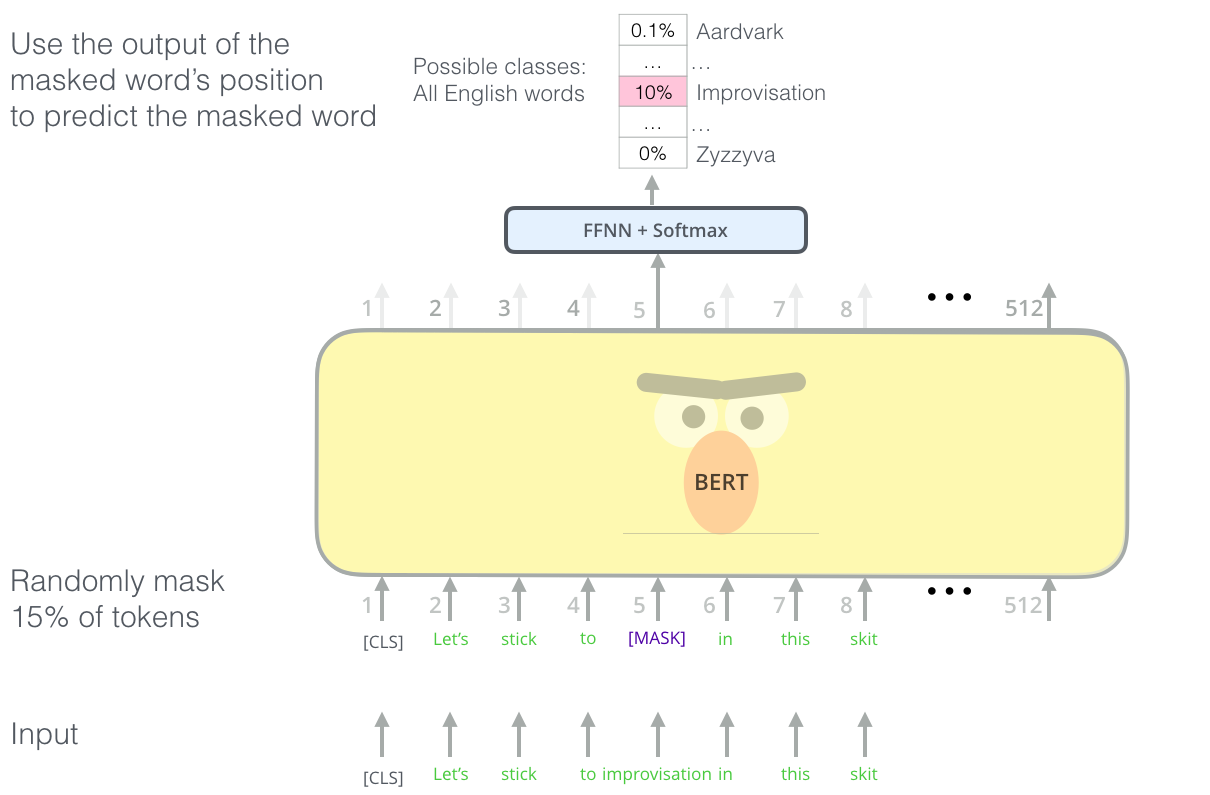
\includegraphics[ width = 1\textwidth]{img/BERT-MLM_3.png}
    \caption{The first task of the self-supervised pre-training process of BERT: Masked Language Modelling. Illustration from~\protect\cite{alammar2018illustrated}}
    \label{fig:BERT_MLM}
\end{figure}


\textbf{Pre-Training - NSP}

In addition to MLM, NSP is used to further improve model pre-training.
For the task of NSP, the model takes two pairs of sentences as input and attempts to predict if the second sentence is subsequent to the first one. In 50\% of the cases, the second sentence of the input pair is the correct subsequent sentence, while in the other 50\%, it is a random sentence from the text corpus.
To solve this task, a [CLS] token is inserted as the first token of the first sentence and a [SEP] token at the end of both sentences. A sentence embedding\footnote{a dictionary of sentence: index letter (A and B)} with a size of 2 (for the two sentences) is used to give information about the sentence order. Moreover, to indicate the position of the token in the sequence, a positional embedding is used. Fig~\ref{fig:BERT_NSP} displays the processes best.
\begin{figure}
    \centering
    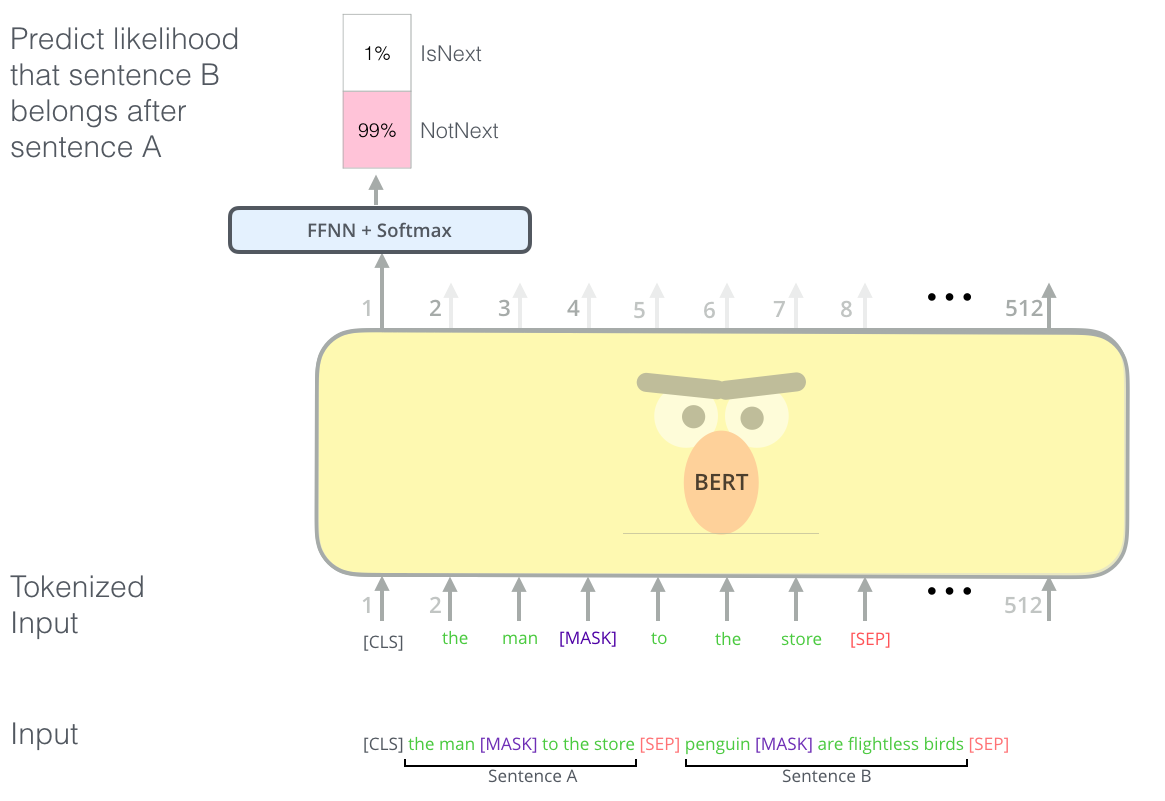
\includegraphics[ width = .9\textwidth]{img/BERT_NSP.png}
    \caption{The second task of the self-supervised pre-training process of BERT: Next Sentence Prediction. Illustration from~\protect\cite{alammar2018illustrated}.}
    \label{fig:BERT_NSP}
\end{figure}

When solving the NSP task, the model first feeds the entire input sequence into the Transformer model, then shapes the output of the [CLS] token into a 2x1 shaped vector and calculates the probability of two sentences being subsequent using the softmax layer.
MLM and NSP are trained simultaniasly while pre-training, which allows for minimizing the combined loss function.

The BERTbase model is pre-trained on a Wikipedia dump and book corpus \cite{zhu2015aligning}, a dataset containing over 10,000 books of different genres. 

Improved versions of BERT vary pre-training tasks and have shown to achieve better performances in certain areas. E.g. the RoBERTa model is pre-trained on the MLM task only \cite{liu2019roberta}. 
 
\textbf{Language Model Fine-tuning}

In fine-tuning for downstream tasks, one or more fully-connected layers are added on top of the pre-trained model's final encoder layer, resulting in a good performance for a broad range of NLP tasks \cite{devlin2018bert}. 

Fine-tuning BERT for down-stream tasks is computationally inexpensive, compared to pre-training. 
The pre-training objectives of MLM and NSP allow it be used on various sequence-pair and single sequence tasks without applying task-specific model architecture alterations. BERT can be fine-tuned on a specific downstream task by swapping out the respective task-specific inputs and outputs. The final step is fine-tuning the parameters end-to-end for an appropriate number of epochs using labeled data from the downstream task. Figure ~\ref{fig:BERT_downstream} shows the fine-tuning of BERT on different downstream tasks. 
At the input, sentence A and B form the pre-training task NSP are comparable with:
\begin{itemize}
\item sentence pairs in paraphrasing
\item hypothesis-premise pairs in entailment
\item question-passage pairs in question answering
\item a degenerate text -$\emptyset$ pair in text classification or sequence tagging.
\end{itemize}

\begin{figure}
    \centering
    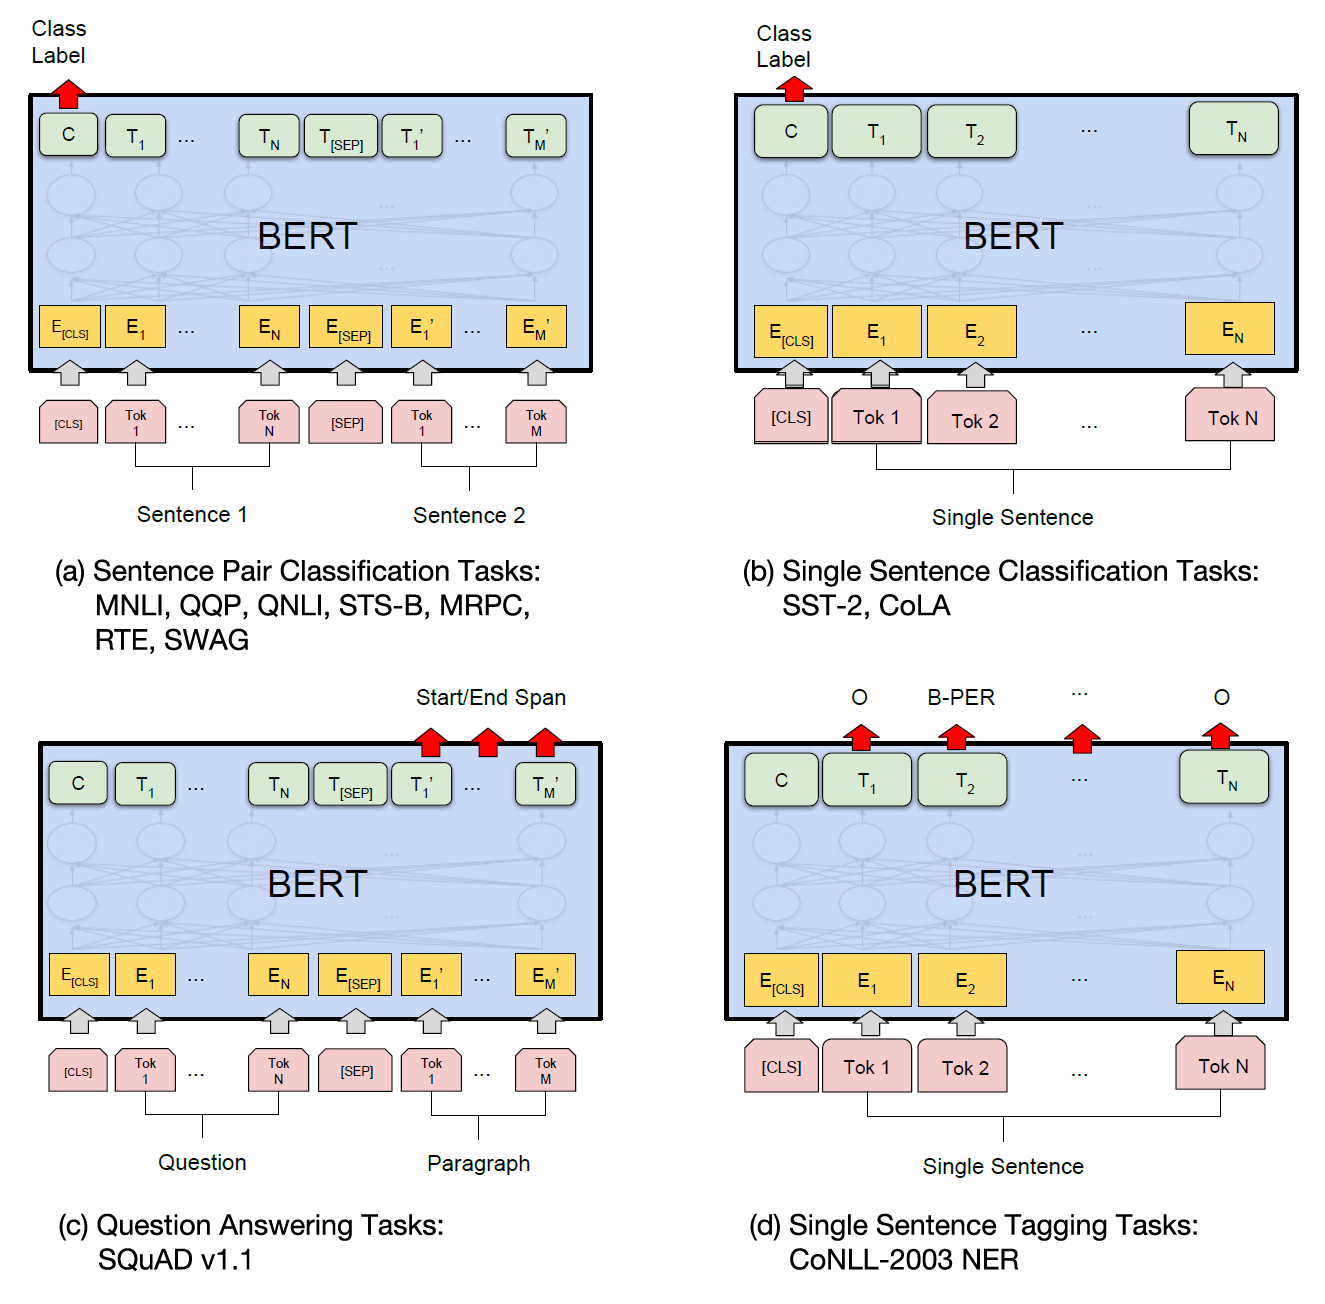
\includegraphics[ width = .9\textwidth]{img/BERT_downstream-tasks.png}
    \caption{Fine-tuning the BERT model on multiple downstream tasks~\protect\cite{devlin2018bert}.}
    \label{fig:BERT_downstream}
\end{figure}


For sequence tagging or question answering, the token representations are fed into an output layer for token-level tasks, while for classification tasks such as entailment or sentiment analysis, the [CLS] token is fed into an output layer for classification \cite{devlin2018bert}. 

\todo{redo adv examples (zum Schluss)}

\begin{figure}
    \centering
    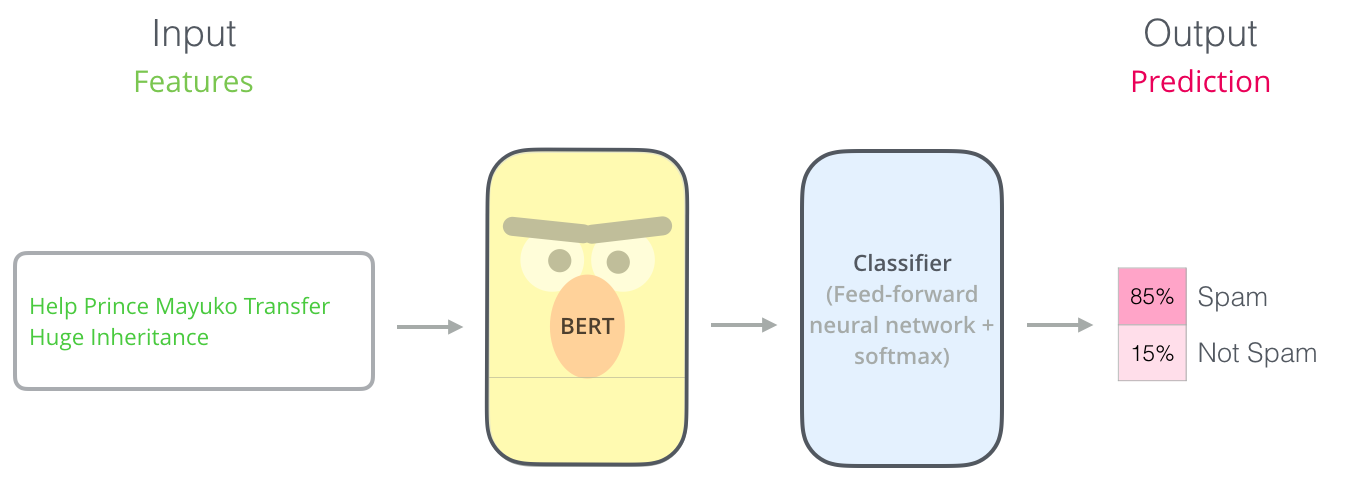
\includegraphics[ width = .9\textwidth]{img/BERT-Finetuning.png}
    \caption{Finetuning of BERT for a simple classification task detecting spam in E-Mails. Illustration from~\protect\cite{alammar2018illustrated}}
    \label{fig:BERT_NSP}
\end{figure}

\subsection{Adversarial Examples}
\label{sec:adversarial_examples}

In 2013, \cite{szegedy2013intriguing} were the first to discover the vulnerability of several machine learning models through adversarial examples: inputs crafted by adversaries with the intent of causing deep
neural networks to misclassify \cite{papernot2016crafting}. These carefully curated examples are correctly classified by a human observer but can fool a target model, raising serious concerns regarding the security of existing machine learning algorithms. 
The altered input data is crafted from a valid sample and either the model's gradients or its output data. 
To describe adversarial examples in a formalized manner, a classifier can be defined as a function \(C(x) = y\). This function has the input value \(x\) and the output value \(y\). After an attacker modifies the input value \(x\), it will become \(x'\), which is incorrectly classified by the algorithm and leads to \(C(x) \neq C(x')\). 
The difference between \(x\) and \(x'\) is commonly called the distance matrix \cite{carlini2017towards}. 
See Figure \ref{fig:advEx} for an example of an applied adversarial perturbation. The image of a panda, which is originally classified correctly with the label "panda" will be misclassified as "gibbon" after adding imperceptible noises. 
\begin{figure}
    \centering
    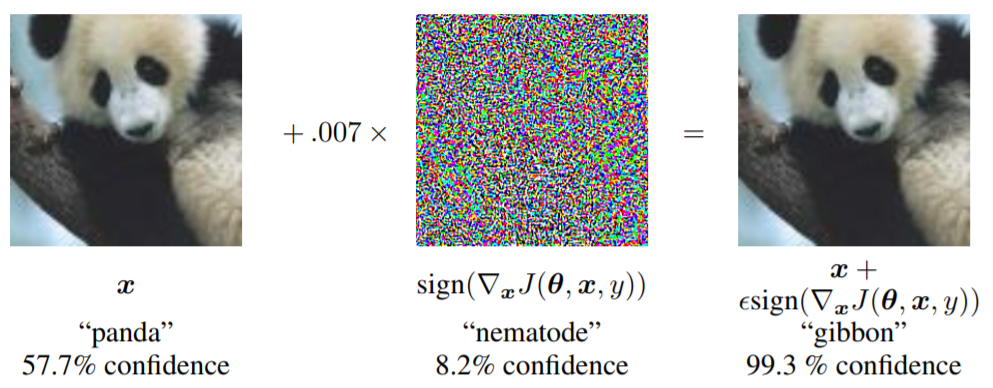
\includegraphics[ width = .8\textwidth]{img/advExample.jpg}
    \caption{Adversarial example in computer vision.~\protect\cite{papernot2016crafting}. Original image of a panda bear shown on the left side. The right side shows the misclassified image with the added perturbation, shown in the middle.}
    \label{fig:advEx}
\end{figure}

The notation "adversarial example" is used in follow-up research to denote all kinds of perturbation samples in a general manner. In further research, \cite{goodfellow2014explaining} found that a wide variety of models with different architectures misclassify the same adversarial example, even when trained on different subsets of training data. Those examples are called transferable adversarial examples. These findings indicate that adversarial examples pose a fundamental blind spot in machine learning algorithms.

\subsubsection{Adversarial Examples in CV}
In research, we distinguish between two types of settings.
An attacker operates either in a black or white-box setting, depending on the degree of access, he or she has to the system. While in a black-box setting, the attacker does not have access to the target model's internal architecture or its parameters, he or she has full access to the target model, its parameters, and input feature representations in the white-box setting. The adversary cannot alter the training data or the target model itself in both cases.

Other works have designed attacks in the "extended white-box" or "gray-box" setting, which describes the scenario of some aspects of the setup being known to the attacker while some are not \cite{vivek2018gray}. However, the definitions for those scenarios seem to vary in the different approaches.

Depending on the purpose of the adversarial attacks, they can be categorized as targeted and non-targeted attacks. While in a targeted attack, the output category of a generated example is intentionally controlled to a specific target category, a non-targeted attack does not take the category of misclassified results into consideration \cite{vijayaraghavan2019generating}.


%-------------------------------------------------------------------
%--------------Adversarial Examples in TEXT-----------------------
%------------------------------------------------------------------
\label{sec:adversarial_exapmles_in_text}

In this thesis, we will further go into the exploratory approach, and, in the following chapter compare adversarial attacks in computer vision with those in NLP and study different approaches proposed so far.

\subsubsection{Differences in Adversarial Attacks for CV and NLP }
\label{sec:differences_in_adv-ex}

Using gradient-based adversarial methods, as used in computer vision, for attacks in the text domain, can result in altered semantics, syntactically-incorrect sentences, or invalid words that cannot be matched with any words in the word embedding space \cite{zhang2019adversarial}. When attacking textual DNNs, it is crucial to carefully design variants or distance measures of the perturbation.

There are three main differences in attacking DNN models for computer vision and natural language processing:

\textbf{1. Discrete vs. continuous inputs}

Typical methods to generate adversarial examples in the image domain use $L_p$ norms to measure the distance between an original data point and a perturbed data one. 
In an image, each pixel has a number representation within a fixed range. A common representation is to use floating numbers in the range ${[0,1]}$ or ${\{0,1,}$\dots${,255\}}$. This indicates that the numerical representation of a pixel gives an insight into the characteristics of the image, and from this, it can be deduced that pixels with similar numerical representations are closely related in terms of their characteristics. The case is different with the numerical representation of word tokens.
Since textual data is symbolic, thus discrete, it is not possible to adapt this in the text-domain, since adopting this method from computer vision often results in altered semantic meaning or syntactically-incorrect sentences. The generation of adversarial examples in the text-domain is therefore considered more challenging\cite{carlini2018audio} 

\textbf{2. Semantic meaning vs. no semantic meaning}

When generating adversarial images, the picture's semantic meaning usually remains unchanged. This is different in the text domain, where a change of a sentence's semantic meaning happens easily. As described in chapter~\ref{sec:word_embeddings}, the mapping from natural language into a corresponding vector is done through the generation of word embeddings.
Given the example sentence, "I like cats", both, the generation of an adversarial example on word-level (e.g., changed word: $cat$ - generated adversarial sentence through word-swap: "I like dogs"), as well as on character-level (e.g., changed character: $t$ - generated adversarial example through character-swap: "I like cars"). Thus, the numerical representation of the word 'cat' might be close to that of the word "dog".
However, that does not mean that the semantic meaning of the words are similar, as it is the case with pixels.


\textbf{3. Perceptible vs unperceivable}

Small modifications of image pixels are hardly recognized by human beings, as shown in Figure ~\ref{fig:advEx}. Hence, if successful, adversarial examples will change the DNNs prediction but not human judgment. Small changes in the text, e.g., character or word modifications, however, are easily detected and, therefore, render the possibility of attack failure. Moreover, a modification can be identified not only by humans but might also be corrected by spelling- or grammar-check systems. Hence, it is not trivial to find imperceivable textual adversarial examples.



\subsection{Adversarial Attacks in NLP}
\label{sec:adv-ex_in_NLP}

In recent years the research motivation to generate adversarial examples in NLP has increased. Jia and Liang were the first to conduct adversarial attacks on textual DNNs and gained attention in the NLP community\cite{Jia2017AdversarialEF}. They addressed the reading comprehension task and showed that they could cause models to output wrong predictions by appending distractor sentences to the end of their input sequences. Inspired by their work, Glockner et al. conducted attacks using the entailment task on the word-level by replacing one word with either a synonym or its hypernym \cite{glockner2018breaking}. Since then, many studies have investigated the security of NLP task DNNs and proposed several attack methods. 
To better compare the numerous different attack methods suggested for NLP models so far, we will use a unified definition framework provided by Morris et al., introduced in their paper on the Software Framework TextAttack for adversarial attacks in NLP\cite{morris2020textattack}. They determine four components, namely a goal function, a search method, a transformation, and an optional list of constraints. In the following chapter, we will explain those components in more detail and assemble attacks from the literature, by means of the components.


\subsubsection{Goal Function}
\label{sec:goal_funciton}
The goal function determines if an attack is finished, given an input $x$. 
The applied parameters are described in the previous sections and include e.g., the attacker's model knowledge and the target class.
An example would be the goal function:

$G(x):= \{argmax$F(x)$ \neq $original\textunderscore class$\}$

for the attack being successful if the prediction after the attack is unequal the original prediction. 

Proposed goal functions in the literature include untargeted goal functions \cite{ebrahimi2017hotflip, alzantot2018generating, li2018textbugger, jin2019bert, garg2020bae}, in the white-box \cite{papernot2016crafting, liang2017deep, ebrahimi2017hotflip, jin2019bert} and the black box setting \cite{gao2018black, goodman2020fastwordbug}.

\subsubsection{Search Method}
\label{sec:search_method}

A search method's aim is to find a perturbation that generates a successful adversarial example and satisfies the constraints. There have been many different approaches introduced for this process over the years. The most popular can be categorized into:

    \textbf{a) Greedy with Word Importance Ranking}
    
        The Greedy approach ranks all words of the input according to some ranking system. The perturbation is then conducted either on the most important word or one at a time in order of decreasing importance \cite{li2018textbugger, jin2019bert, garg2020bae}.
    
        Liang et al. were the first to enhance their attacks' efficiency by introducing a two-step approach to generate adversarial attacks in text. They first determine the text items essential for their classification by computing the cost gradient of the input (white-box), as well as generating a series of occluded test samples (black-box attack)\cite{liang2017deep}. 
        Since the adversary in a black-box setting does not have any indication of where the model could be prune to attacks, a two-step approach is required to enhance the efficiency by not having to try all possible modifications or to attack randomly chosen words. 
        In their paper, Gao et al. used the two-step approach. They first determine the words critical for the model's prediction by introducing a word importance scoring function. In a second step, they generate adversarial text by making imperceptible edit operations to the word previously determined 'important' words, forcing the classifier to make wrong predictions \cite{gao2018black}.
        In 2019, the pre-trained BERT model was attacked by adversarial examples for the first time by Jin et al. They conducted a word importance ranking by analyzing the prediction change before and after deleting one word, also called Leave-One-Out Method.  
        
        \textbf{Leave One Out Method for Important-Word-Detection}
        

        Leave One Out is an interpretation method used to determine the words of a document that contribute most to the output of a model prediction. The effort to create a successful adversarial example can be minimized by targeting the attack on the word with the strongest influence on the prediction outcome. The leave one out method resembles a process that iteratively removes one word after another and predicts each sentence without the removed word. 
        This way, a document consisting of e.g., ten words, is sent through the Machine Learning Model eleven times. (Once the complete sentence is predicted, then without the first word, without the second word, and so on). The words which changed the model's prediction of the sentence, through their absence, are considered important words. 
        
    \textbf{b) Beam Search}
    
        Ebrahimi et al., introduced HotFlip, a method to generate adversarial examples with character substitutions, using the gradient with respect to a one-hot input representation, aiming to determine the individual change with the highest estimated loss. They use the beam search to find a set of manipulations that fool the classifier best when conducted together \cite{ebrahimi2017hotflip}. The Beam Search initially scores transformations at all positions in the input and ascertain the top b transformation (where b is a hyperparameter known as the "beam width"). After that, it iterates, looking at transformations of all sequences in the beam \cite{tillmann2003word}. 
        
    \textbf{c) Genethic Algorithm}
    
        Alzatot et al. were the first to use the genetic algorithm as a search method. Instead of relying on gradient-based optimization, they developed an attack algorithm that exploits population-based gradient-free optimization through genetic algorithms. Genetic algorithms are inspired by the process of natural selection, iteratively evolving a population towards better solutions. They determine the best solution through a combination of crossover and mutation. That way, they can find successful adversarial examples with fewer modifications \cite{alzantot2018generating}.
        
        
\subsubsection{Transformation}
\label{sec:transformation}
    The transformation takes an input and returns all potential perturbations while being agnostic of goal function and constraints. Transformation methods can be categorized according to the attacker's model knowledge (white-box and black-box).

    Papernot et al. were the first in 2016 to generate adversarial examples in text. They investigated on adversarial inputs for RNNs processing sequential data using the Fast Gradient Sign Method (FGSM) to generate adversarial sequences in the white-box setting \cite{papernot2016crafting}. 
    Gradient calculations are used to determine which features have to be modified to generate an adversarial example. The method is very effective for generating adversarial examples in the field of computer vision \cite{goodfellow2014explaining}.
    Papernot et al. found that switching from computer vision to natural language processing applications using the FGSM introduced difficulties (as explained in the previous chapter). 
    Goodman et al. generated small utility-preserving text perturbations in a black-box setting by using a scoring method to identify important words that affect text classification \cite{goodman2020fastwordbug}, similar to Gao et al., who, in 2018, use a scoring strategy to generate character-level transformations in the black-box setting on RNN based natural language classifiers. They conduct small edit operations to a text sequence such that a human would consider it similar to the original sequence. They do this by first targeting the important tokens in the sequence and then execute a modification on those tokens that can force the classifier to make a wrong prediction. They perturb using four methods, namely substitution of a letter in a word with a random letter, deletion of a random letter, insertion of a random letter, and swapping two adjacent letters. Their method achieves better results than FGSM  and finds that the selection of words to perturb is more important than the alteration of words\cite{gao2018black}.  In 2017 Liang et al. were able to successfully fool character- and word-level DNN-based text classifiers through the conduction of three perturbation strategies, namely insertion, modification, and removal \cite{liang2017deep}. In 2019, Jin et al. were the first to attack the pre-trained BERT model. Their perturbation approach is word-level based, as they replace the original word with synonyms and use word embedding vectors to measure how well different models judge the semantic similarity between the words \cite{jin2019bert}.
    
    
\subsubsection{Constraints}
\label{sec:constraints}
    When conducting modifications on a textual input sequence of an NLP model, it is likely to alter the semantic meaning or grammatical correctness. E.g.,  the FGSM method to generate modified input. There is no guarantee that words close in the embedding space are semantically similar. Therefore, this approach may replace words with semantically different others and might alter the whole sentence's semantics.
    
    An attack is considered valid if the input satisfies each of the attacker's constraints. 
    Constraints include different approaches. One approach is to measure the edit distances, e.g., the maximum percentage of words changed \cite{ebrahimi2017hotflip} or maximum Levenshtein edit distance \cite{gao2018black}. Samanta et al. use saliency maps to ensure semantically meaningful adversarial examples\cite{samanta2017towards}. This approach, however, is difficult to perform automatically. Grammatically constraints are intended to prevent the attack from creating perturbations that introduce grammatical errors. Examples here are Part-of-speech consistency or a maximum number of grammatical errors \cite{ebrahimi2017hotflip, jin2019bert}. Semantics constraints aim to preserve the meaning between $x$ and $x\textunderscore adv$, e.g., maximum swapped word embedding distances, or using sentence encoders or language models \cite{cer2018universal, garg2020bae, jin2019bert, li2018textbugger, alzantot2018generating, ebrahimi2017hotflip}.


%-------------------------------------------------------------------
%-------------------------------------------------------------------
%-----------------------------Methodology--------------------------
%-------------------------------------------------------------------
%-------------------------------------------------------------------

\section{Methodology}
\label{sec:methodology}

Building on the theoretical foundations laid out in the previous section, we will now determine areas of the current state of research that have not yet been examined. Drawing on that we will develop the research question and explain the methodology used in the practical part of the work to answer the it. 


\subsection{Objectives todo}
\label{sec:objectives}
- what objectives
- rq

In our thesis we wanted to determine the robustness of the famous BERT model and, hence find out if it can be fooled by minor changes. The aim of the work was answer the following research question:

RQ1: How robust is BERT based NLP model for the task of ABSA against input level adversarial examples?

Our experiments will result in datasets containing adversarial examples.

Later on, we will try to generate examples by modifying these words.
The prediction is considered changed as soon as one of the three output categories (entity, attribute, or sentiment) is changed by omitting a word. ]

%-------------------------------------------------------------------
%-------------------------Setup -----------------------------
%------------------------------------------------------------------

\subsection{Experimental Setup} 
To answer our research question, we conducted three input character-level adversarial attacks against the prominent pre-trained BERT model introduced by Google in 2018. 
We evaluated the robustness of our model in an in-domain classification task, called ABSA. As described before, the ABSA task refers to the prediction of an aspect mentioned in an input sequence and the corresponding sentiment. ABSA is considered a multilabel task, since $[0,1, \dots n]$ labels can be predicted for one input sequence. 

To better illustrate our proceedings, we draw on the proposed framework by Morris et al.:

Our \textbf{goal function} is represented by the following formula: ${f( x_adv ) = y_adv \neq y}$. It is described in more detail in section~\ref{sec:experiments}

The \textbf{Search Method} used in this thesis is called Leave-One-Out (LOO) and discussed in section~\ref{sec:iwd_method}.

\textbf{Transformations} are conducted on the character-level rather than the word-level and elaborated on in section~\ref{sec:attacks_method}.

To determine \textbf{Constraints} and how our attacks are evaluated, see section~\ref{sec:evaluation_tb}.

\subsubsection{Attacks}
\label{sec:attacks_method}
As most existing approaches generate adversarial examples as attacks by finding the minimum perturbation \cite{liang2017deep, ebrahimi2017hotflip, gao2018black, li2018textbugger, alzantot2018generating, jin2019bert, garg2020bae}, the attacks tend to be conspicuous and can easily be identified by humans. Moreover, they are not likely to appear in nature, making them less relevant in practical applications. Perturbations are either word or character level based. Possible variations have been proposed in the literature and are described in chapter ~\ref{sec:adversarial_exapmles_in_text}. Examples are randomly replacing, deleting, swapping, or inserting characters. Perturbations on the word level basis use the same example approaches.  
The disadvantage of word-level perturbations is that an unintentional change of the semantic meaning of a sentence is likely to happen. This means that the comparison of a sentence's prediction before and after the change of a word is no longer guaranteed, which poses a constraint. Various methods have been proposed to avoid this problem and are described in section \textbf{Constraints} in chapter ~\ref{sec:adversarial_exapmles_in_text}. 
This phenomenon occurs less often when perturbing on the character level since the perturbed words remain the same. An exception is when the change of single characters randomly results in a new, existing word of the dictionary with a different semantic meaning. 
To prevent humans from easily identifying our attacks as adversarial examples, we propose three character-level attack methods that are likely to occur in a practical scenario. The attacks can be subdivided into three attack methods:


\textbf{Leet speak}

Leet speak (or '1337') is a system of modifying spelling, primarily used in online games, internet platforms as well as in the 'hacker'-community. The term 'leet' derives from the word 'elite' and describes the communities that use it. The purpose of using leet speak can be to exclude newcomers (e.g., in an online community or game) or outsiders in general. The goal is to create language, that the average reader cannot make sense of \cite{thomas2002hacker}.
Leet speak is characterized by the use of non-alphabet characters to substitute one or multiple letters of one word with visually similar-looking symbols, so-called homoglyphs. Commonly used homoglyphs in leet speak are numbers. 
We conducted experiments to explore the effect of leet speak on the BERT model. As described in chapter~\ref{sec:the_history_of_NLP} DNN-based text classification continuously gains importance for enhancing the safety of online communication e.g., in online discussion environments through toxic content detection and other methods \cite{kumar2011natural}. This are the environments where leet speak is used commonly. The investigation of what effects the character substitution has on the used BERT models could help to increase safety in such forums and other environments where users use this language. 

\textbf{Spelling mistakes}

As described, the BERT base model is pre-trained on Wikipedia and book corpus \cite{zhu2015aligning}, a dataset containing over 10,000 books of different genres. Since it is used for different use cases, of which many include the processing of user-generated data, the BERT model should be robust against spelling mistakes. Sun et al., were the first in 2020 to study the effect of spelling mistakes on the BERT model using different methods \cite{sun2020adv}. Just like them, we will make use of the list of common misspellings generated by Wikipedia\footnote{\url{https://en.wikipedia.org/wiki/Wikipedia:Lists_of_common_misspellings}} to generate adversarial examples. The difference to their work is the method for identifying the word to execute the perturbation on. 
The words in the list are gathered by users reporting misspellings. A misspelling is considered common and added to the list if it occurs in Wikipedia at least once a year.
The list consists of 4282 entries, where one word can have multiple misspelling variations. 


\textbf{Punctuation}

To the best of our knowledge, there have not been any investigations on the effect of changed punctuation symbols on the robustness of a BERT model. Since we were able to generate successful attacks by merely adding one punctuation mark, we limited ourselves to that and did no further research on different punctuation variations. Moreover, one additional comma is unobtrusive, occurs in the practical use cases, and is not easily identified as an adversarial example by a human observer.


\subsubsection{Target Model} 
\label{sec:target_model_method}

As the base for our experiments we used the uncased BERTbase model\footnote{\url{https://huggingface.co/bert-base-uncased}}\cite{DBLP:journals/corr/abs-1810-04805}. In a first step, pre-trained it on the laptop domain and in a second step, fine-tuned in on the ABSA task. In pre-training, BERT solves the two calssification tasks MLM and NSP usually on a large corpora of unlabeled text. We use Amazon Laptop Reviews scraped by He et. al. \cite{he2016ups}. We used the Adam optimizer and 32 bit floating points computations. Adam is an optimization method used to update network weights iteratively in the training process of deep learning models. This optimizer, being a replacement for the stochastic gradient descent, is commonly used since it comes with a straight-forward configuration process and default parameters are suitable for most tasks \cite{kingma2014adam}. We pre-train our model using a batch size of 32 and set the learning rate to 3 $*$ 10$^{-5}$.
We define a maximum input sequence length of 256 tokens, resulting in four sentences per sequence on average.  Due to the relatively low number of training data, we pre-train BERTbase for 30 epochs, so that the model sees about 30 million sentences during training. That way, a single sentence appears multiple times within the two language model tasks. Please find the code for pre-training on GitHub, to reproduce the langauge model\footnote{\url{https://github.com/deepopinion/domain-adapted-atsc}}.

For fine-tuning the pre-trained BERT model on the ABSA task, we, again, used 32 bit floating point computations, the Ranger optimizer and set the learning rate to 4 $*$ e$^{-5}$. We used a batch size of 32 and fine-tuned it for 20 epochs and random initialization. While the training loss improved continuously, validation accuracy converges already after the xxth epoch of training. Our experiments are based on the model at the xth ... 
\todo{check!}


For tokenization we used the \texttt{PreTrainedTokenizer} introduced with the BERTbase model\footnote{\url{https://huggingface.co/transformers/main_classes/tokenizer.html}}. The library includes the following methods:
\begin{itemize}
\item tokenization of string input and converting token strings to ids and back,
\item adding new tokens to the vocabulary and
\item managing special tokens.
\end{itemize}


\subsubsection{Important Word Detection}
\label{sec:iwd_method}
As mentioned in section ~\ref{sec:adversarial_exapmles_in_text}, the two-step approach to conduct adversarial examples in the text domain is an effective method commonly used in research. The two steps are: firstly, determining the words which have a critical influence on the model's prediction and secondly, perturbing the identified important words. This approach allows for effective fooling of the target classifiers and minimizing the input modification effort \cite{jin2019bert}. Several methods to determine the important word have been proposed in literature.
In 2018 Feng et al. introduced input reduction, a method to enhance the interpretation of neural models \cite{feng2018pathologies}. They aim to find a subset of the most important words of an input sequence that contributes most to a prediction by resembling a process that iteratively removes 'unimportant' words for the input until the prediction of the model changes. The remaining set of words before the predictions changes are considered critical for the prediction output. To decide on which words to remove, they compare the prediction probability towards the original label of a sentence containing the word with the prediction probability of a sentence where the same word was removed. This method is called Leave One Out (LOO) and can itself be used as an approach to determine the important word of an input sequence. The LOO method was introduced by Vehtari et al. to estimate pointwise out-of-sample prediction accuracy \cite{vehtari2017practical}. 

% Important word detection
Given an input sentence $\textbf{x}$ represented as a list of word tokens ${\textbf{x} = [x_1, x_2,}$ \dots${x_n]}$ and a predicted output label $y$. The important word is defined as 
.....
\todo{formula überlegen}

In different terms, the importance of a word is determined by comparing the output label $y$ with the ...

This formula is applied for every word token $x$ in a input sequence to determine all words influential to the prediction. Therefore, one input sequence can contain $[0,1, \dots n]$ important words. 
Comparing the prediction before and after a word is removed reflects how the word influences the classification result. This procedure allows for enhanced efficiency of adversarial attacks in the text domain.


\subsubsection{Datasets} 
\label{sec:datasets}
We conduct our experiment using SemEval-2015 Task 12: Aspect Based Sentiment Analysis dataset for the laptops domain \cite{pontiki2015semeval}. An aspect category is defined as a conbination of an entity type $E$ and an attribute type $A$. E describes the reviewed entity (e.g. laptop), while A describes a particular attribute of E (e.g. durability or quality).
To give an example:
Given the review \textit{"They sent it back with a huge crack in it and it still didn't work; and that was the fourth time I've sent it to them to get fixed"}, E could be \textit{customer support} and A could be \textit{quality}. The third slot is used to determine the sentiment polarity towards the entity and its attribute (\textit{positive, neutral or negative}). The sentiment for the above given example would be \textit{negative}.
The three slots are linked to each other within tuples. For this thesis we decided to use only one of the three provided domains, namely Laptops. The Laptop dataset contains 1,739 sentences in the training data and 761 sentences in the test data set. Figure ~\ref{fig:semeval} provides a table of entity and attributes labels, used in the dataset.

\begin{figure}
    \centering
    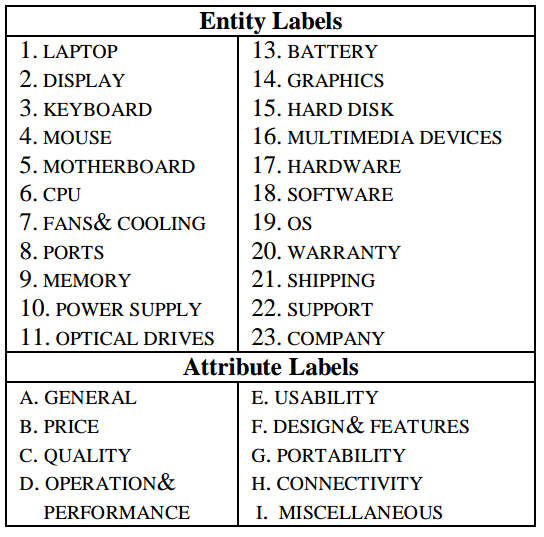
\includegraphics[ width = .5\textwidth]{img/semeval.png}
    \caption{Laptop Entity Aspect Categories~\protect\cite{pontiki2015semeval}.}
    \label{fig:semeval}
\end{figure}

To pre-train the BERT language model on the laptop domain, we use Amazon Laptop reviews \cite{he2016ups}. To avoid training bias for the SemEval-2015 test data, we filtered out reviews that appeared in both, the Amazon and the SemEval Test Dataset. Moreover, we removed reviews that contain less than two sentences from the training corpora, to achieve compatibility with the NSP task used for fine tuning. After the text pre-processing there are 1,007,209 sentences left in the corpus. 



\subsection{Evaluation Criteria todo}
    \label{sec:evaluation_tb}
As described in chapter~\ref{sec:adversarial_exapmles_in_text} there are a number of methods proposed to generate adversarial examples in the text domain. Since it is not trivial to assess the quality of these different attacks, as small perturbations can lead to significant changes in semantics meaning of the textual input. In their paper, Xu et al. propose Elephant in the Room, an evaluation framework to assess the quality of adversarial examples in the text domain\cite{xu2020elephant}. Their (automatic) evaluation criteria are:
(a) attacking performance (i.e. how well they fool the classifier); 
(b) textual similarity between the original input and the adversarial input; and
(c) fluency of the adversarial example.

More approaches on the evaluation of adversarial attacks in the text domain are explained in section ~\ref{sec:constraints}. In order to guarantee the constraints, more or less effort must be made, depending on the evaluation method. Some semantic, and grammatical evaluation methods can be performed using additional DNN-based classifiers \cite{ebrahimi2017hotflip, jin2019bert, garg2020bae}.

Other constraints, e.g. to ensure remaining semantic meaning, or to preserve context fitting, can be evaluated by humans only. 
Common ways to evaluate the effectiveness of adversarial attacks are the determination of F-Scores and accuracy for whole datasets, or confidence levels for single predictions. 

by design!!!!!!!!


\section{Experiments todo}
\label{sec:experiments}

The experiments in this thesis are conducted in the black-box setting, as there is no knowledge about the model architecture or the training data needed. Since there is more practical relevance for this scenario, we will conduct non-targeted attacks and focus on the input level rather than the embedding or semantic level to execute our perturbations. 
By design, we chose our attacks in a way, that a human observer would not be able to identify them as adversarial attacks. 

To limit the scope of this work, we refrain from reviewing the semantic meaning of the generated adversarial sentences.
As described, adversarial attacks in computer vision differ from the ones in the text domain and are therefor considered more challenging. We adapted the two-step approach introduced in the literature and were able to enhance efficiency. 
....

\subsection{Goal Function}
 \label{sec:goal_function_m}
We have the pre-trained BERTbase language model $f$: ${X \rightarrow Y}$ for the task of ABSA, where $X$ are the input text sequences, and $Y$ are the corresponding labels consisting of E entity, A attribute, and S sentiment. We generate adversarial examples ${x_adv}$ from the original input $x \in X$, and the original prediction $y \in Y$. We do this by determining the important word $i$ of a sequence and replacing it the modified word $i_adv$. Since we aim for changing the model's prediction, our goal function is the following: 
$f$( $x_adv$ ) = $y_adv$ \neq $y$.


To conduct the experiments we used the described SemEval 2015 dataset conatining 1971 reviews on laptops. Before working with the data, we converted it in an adequate format and filtered for unique sequences, resulting in a dataset of 1396 items in the following format:
\todo{same example for whole thesis}
\texttt{['This computer is absolutely AMAZING!!!', '10 plus hours of battery...']}


\subsection{Search Method}
\label{sec:search_method_m}
Since we operate in the black box setting and therefore do not have access to prediction probability values, as needed for the input reduction method, we make use of the LOO-method to determine the words of a sequence critical for the output of the model's prediction. That way can ascertain which word to place our attack on, in order to achieve maximal efficiency. The theoretical basics of the method are discussed in section ~\ref{sec:iwd_method}.
First, we predicted the 1396 original examples and stored the labels. After that we tokenized the examples by creating a list for each sequence containing the respective words. In the next step, we iterated over the lists of words in a sequence and removed the respective word in the original sentence. We repeated this step for each word in the original sentence. 
After this process, we have as many modified sentences as we have original times the respective number of words. A word is considered important, if it's omission triggered a flip in the prediction, compared to the original sentence. 
In 943 sequences, we were able to find 1 or more important words. The cumulative number of successful modifications caused by the LOO-method 2694. In other words, one sequence contains 1.93 important words on average.

\subsection{Transformation}
\label{sec:transformation_m}
In section ~\ref{sec:attacks_method} we proposed three attack methods and discussed the theoretical background. We now elaborate on the technical implementation, carried out to generate adversarial examples.

\textbf{Leet Speak}

To generate leet speak, we take the important words of a sentence and apply the function below. That way we swap the letters a, e, l, o, and s with the numbers 4, 3, 1, 0, and 5 respectively. We limited ourselves to this 5 characters in order to preserve the readability. 
\definecolor{dkgreen}{rgb}{0,0.6,0}
\definecolor{gray}{rgb}{0.5,0.5,0.5}
\definecolor{mauve}{rgb}{0.58,0,0.82}

\lstset{frame=tb,
  language=Python,
  aboveskip=3mm,
  belowskip=3mm,
  showstringspaces=false,
  columns=flexible,
  basicstyle={\small\ttfamily},
  numbers=none,
  numberstyle=\tiny\color{gray},
  keywordstyle=\color{blue},
  commentstyle=\color{dkgreen},
  stringstyle=\color{mauve},
  breaklines=true,
  breakatwhitespace=true,
  tabsize=3
}
\begin{lstlisting}
def to_leet(word):
    getchar = lambda c: chars[c] if c in chars else c
    chars = {"a":"4","e":"3","l":"1","o":"0","s":"5"}
    return ''.join(getchar(c) for c in word)
\end{lstlisting}
Of a total of 943 sequences, we were able to modify 897 resulting in 2232 cumulative modified sequences. This means, in 46 sentences, the important words did not contain the letters a, e, l, o, or s, and we therefore could not swap a letter with a number.
After the modification, we predicted the modified sequences and compared the prediction with the prediction of the original sequences. 

\texttt{original\_sentence: "super fast processor and really nice graphics card..",
modified\_sentences: 
"super f45t processor and really nice graphics card..", 
"super fast pr0c3550r and really nice graphics card.."]}

\textbf{Spelling Mistakes}

To generate adversarial examples containig spelling mistakes we used the Wikipedia corpus of typos described in section ~\ref{sec:attacks_method}. We went over the important words in a sequence and checked in the dictionary, if it contained one or more entries of it. For 369 of 943 sequences we were able to find at least one modification for at least one important word, resulting in 1354  modified sequences in total.
The example below illustrates an example. The important word determined in this sentence is "condition". The typo list contains one entry for the word "condition", being "condidtion". 

\texttt{original\_sentence: "It is the best condition and has a really high quality.",
modified\_sentence: "It is the best condidtion and has a really high quality.}


\textbf{Punctuation}

The third attack method was initially planned to be more complex, since we realized, that even a simple modification effects the classifier tremendously. For our attack, we added a comma after the important word. 
\definecolor{dkgreen}{rgb}{0,0.6,0}
\definecolor{gray}{rgb}{0.5,0.5,0.5}
\definecolor{mauve}{rgb}{0.58,0,0.82}

\lstset{frame=tb,
  language=Python,
  aboveskip=3mm,
  belowskip=3mm,
  showstringspaces=false,
  columns=flexible,
  basicstyle={\small\ttfamily},
  numbers=none,
  numberstyle=\tiny\color{gray},
  keywordstyle=\color{blue},
  commentstyle=\color{dkgreen},
  stringstyle=\color{mauve},
  breaklines=true,
  breakatwhitespace=true,
  tabsize=3
}
\begin{lstlisting}
def to_punctuation(word):
    return ''.join((word, ','))
\end{lstlisting}

That way we were able to modify 943 out of 943 sequences, resulting in 2555 modified sequences in total. 

\subsection{Constraints and Evaluation}
    \label{sec:constraints_m}
~~~vage~~

We evaluate our experiments using two of Xu et al.'s proposed evaluation criteria mentioned in section ~\ref{sec:evaluation_tb}. 

\textbf{Attacking Performance}

We consider a an adversarial example successful, if we were able to switch the prediction of a sentence $s$, resulting in ${f(x_adv ) = y_adv \neq y}$.
We consider ${y_adv \neq y}$ if we were able to change one, or more of the three prediction-parts for a sentence $s$: E entity, A attribute, or S sentiment. 
A prediction can be changed in three different ways:
\begin{itemize}
\item a different E, A or S is predicted,
\item the model does no longer predict a label, or
\item the model predicts a label, when it did not predict one before.
\end{itemize}

\textbf{Textual Similarity between $x$ and $x_adv$}

\textbf{Leet}
\textbf{Typo}
\textbf{Punctuation}


As described in their paper, it involves a great deal of effort to ensure (b) textual similarity between the original and adversarial input and (c) the fluency of the adversarial example.
.. word-level

By design we chose attacks that are supposed to fool the human prediction. The the

\subsection{Results todo}
We compare the results of three different attacks, described in seciton~\ref{sec:transformation}. To answer our research question, we can see the results of our experiments in table~\ref{tab:results-table}, which show that the BERT model is \textbf{not} robust against adversarial input on character-level in the black-box setting.
The most successful method, according to our results, is \textbf{Leet Speak}. With it, we were able to achieve a success rate of 47.8\%. As described above, we applied our attack to 2232 sentences and thus triggered a change in prediction for 1066 sentences. By using \textbf{misspellings}, we were able to generate an incorrect prediction for 420 out of 1354 modified sentences, giving a success rate of 31\%. By simply adding one comma behind the important word, we were able to change the prediction for 15\% of the sentences, using the p\textbf{unctuation method}.  Out of 2555 sentences, we got a modified prediction of the model for 382 sentences.
To look into our results in more detail table~\ref{tab:ex_sentence_gaming} shows an example sentence. In this case, we were able to flip the model's prediction using each of the three proposed transformations.

As described, our Aspect-Sentiment pairs look like this:

\texttt{\{"aspect\':\'CPU\#OPERATION\textunderscore PERFORMANCE\', \'sentiment\': \'POS\'\}}.

They consist of three parts:
\begin{itemize}
\item Entity (e.g. 'CPU')
\item Attribute (e.g. 'OPERATION\textunderscore PERFORMANCE')
\item Sentiment (e.g. 'POS')
\end{itemize}

The table shows the example sentence "It's wonderful for computer gaming" with the original prediction result LAPTOP\#MISCELLANEOUS POS. Our search method revealed the word, decisive for the sentence's prediction is "wonderful". Note that this is the only important word in this sentence. The word "wonderful" was, depending on the attack method, transformed into "w0nd3rfu1", "wonderfull", and "wonderful,". We were able to change the result of the prediction by using any of the methods. In this example, the correct aspect was identified in all three cases, and the model was able to determine the sentiment correctly despite the modified important word. However, additional aspects were falsely predicted. 

\begin{table}[]
\centering
\resizebox{\textwidth}{!}{%
\begin{tabular}{|c|c|c|c|}
\hline
\rowcolor
Perturbation Method                                      & Leet Speak           & Misspellings         & Punctuation          \\ \hline
Tokenizer                                                & en\_core\_web\_sm    & en\_core\_web\_sm    & en\_core\_web\_sm    \\ \hline
Model                                                    & en\_laptops\_absa    & en\_laptops\_absa    & en\_laptops\_absa    \\ \hline
Dataset                                                  & SemEval 2015 Laptops & SemEval 2015 Laptops & SemEval 2015 Laptops \\ \hline
Total number of original sentences                       & 943                  & 943                  & 943                  \\ \hline
Total number of modifyable original sentences            & 897                  & 369                  & 943                  \\ \hline
Total number of modified sentences                       & 2232                 & 1354                 & 2555                 \\ \hline
Total number of changed predictions through modification & 1066                 & 420                  & 382                  \\ \hline
Success Rate                                             & 0.477599             & 0.310192             & 0.149511             \\ \hline
\end{tabular}%
}
\caption{Results of the three attack methods compared.}
\label{tab:results-table}
\end{table}
% Please add the following required packages to your document preamble:
% \usepackage{graphicx}
% \usepackage[normalem]{ulem}
% \useunder{\uline}{\ul}{}
\begin{table}[]
\centering
\resizebox{\textwidth}{!}{%
\begin{tabular}{|c|l|l|l|}
\hline
\multicolumn{1}{|l|}{\textbf{}} &
  \multicolumn{1}{c|}{\textbf{Sentence}} &
  \multicolumn{1}{c|}{\textbf{ENTITY\#ATTRIBUTE}} &
  \multicolumn{1}{c|}{\textbf{Sentiment}} \\ \hline
\textbf{original} & It's wonderful for computer gaming. & LAPTOP\#MISCELLANEOUS & POS \\ \hline
\textbf{leet} &
  It's w0nd3rfu1 for computer gaming. &
  \begin{tabular}[c]{@{}l@{}}LAPTOP\#GENERAL\\ LAPTOP\#MISCELLANEOUS\\ LAPTOP\#QUALITY\end{tabular} &
  \begin{tabular}[c]{@{}l@{}}POS\\ POS\\ POS\end{tabular} \\ \hline
\textbf{typo} &
  It's wonderfull for computer gaming. &
  \begin{tabular}[c]{@{}l@{}}LAPTOP\#GENERAL\\ LAPTOP\#MISCELLANEOUS\end{tabular} &
  \begin{tabular}[c]{@{}l@{}}POS\\ POS\end{tabular} \\ \hline
\textbf{punctuation} &
  It's wonderful, for computer gaming. &
  \begin{tabular}[c]{@{}l@{}}LAPTOP\#GENERAL\\ LAPTOP\#MISCELLANEOUS\end{tabular} &
  \begin{tabular}[c]{@{}l@{}}POS\\ POS\end{tabular} \\ \hline
\end{tabular}%
}
\caption{Example Sentence modified using the three attack methods leet speak, misspelling, and punctuation.}
\label{tab:ex_sentence_gaming}
\end{table}

\subsubsection{Entity}
With the leet speak method, we were able to change each entity at least once. Unlike the typo method, we could not change the entities 'GRAPHICS', 'BATTERY', 'PORTS', 'SHIPPING', 'FANS\textunderscore COOLING', 'MEMORY', 'HARD\textunderscore DISC', 'KEYBOARD', and 'MOTHERBOARD'. With the punctuation method, we were able to change all entities except the following ones: 'MULTIMEDIA\textunderscore DEVICES', 'KEYBOARD', 'SHIPPING', 'MEMORY', 'HARDWARE' and 'WARRANTY'. 
The ten entities that could be changed most often using the leet method are 'LAPTOP', 'DISPLAY', 'BATTERY', 'KEYBOARD', 'SOFTWARE', 'MOUSE', 'COMPANY', 'MULTIMEDIA\textunderscore DEVICES', 'GRAPHICS', 'SUPPORT'. For the misspelling method, these ten were 'SOFTWARE', 'SUPPORT', 'OS', 'LAPTOP', 'COMPANY', 'CPU', 'MULTIMEDIA\textunderscore DEVICES', 'POWER\textunderscore SUPPLY', 'DISPLAY' and HARDWARE', and for the punctuation method it was 'BATTERY', 'COMPANY', 'LAPTOP', 'SUPPORT', 'OS', 'POWER\textunderscore SUPPLY', 'DISPLAY', 'MOUSE', 'SOFTWARE' and 'HARD\textunderscore DISC'. The order of the enumerations gives indication of the frequency of the changes, with the first named entity being the most frequently changed. The corresponding graphics can be found in the appendix figures ~\ref{fig:entity_change_leet}, ~\ref{fig:entity_change_typo}, and ~\ref{fig:entity_change_punct}. 
We can conclude from this that the entities have been changed at different times.  Interestingly, we cannot detect any entities that are equally robust or susceptible to all three methods. Only the entity 'LAPTOP' was changed most often by the leet method, fourth by the misspelling method, and third most often by the punctuation method. It is also noteworthy that the entity 'BATTERY' is seemingly very susceptible to method 3, punctuation, by which it was changed most frequently, while for the leet method the entity is changed only third most frequently and with the typo method the entity is not even among the ten most frequently changed. This indicates the good robustness of this entity against method two, misspelling. 

\subsubsection{Entity-Attribute}
These observations are similar when we add attributes to the analysis. Using the leet-speak method, we were able to change all except 6 out of 184 possible entity-attribute pairs. This was considerably more challenging with the methods misspelling and punctuation. Here, the lists of entity-attribute pairs that we could not change through modifications are longer. For misspellings, we could not find any changes for 32 entity-attribute pairs. For punctuation, we could not change the entity-attribute prediction of 24 pairs. The respective illustrations show the changes of entity-attribute pairs split respectively and can be found in the appendix figures ~\ref{fig:entity_attr_change_leet}, ~\ref{fig:entity_attr_change_typo}, and ~\ref{fig:entity_attr_change_punct}.

\subsubsection{Entity-Attribute-Sentiment}
Including the predicted sentiment in our evaluation, we see that some entity-attribute-sentiment sets are very susceptible to changes in any of our three methods. For example, the set 'LAPTOP#GENERAL POS' was changed 103 times by leet speak modifications, 48 times by misspellings, and 14 times by added punctuation. This set appeared in the dataset of changed modifiable original sentences 134 times. We could not change all 552 possible combinations of an entity, attribute, and sentiment, whereby the first method is the most efficient. When attacking with the leet method, only 21 sets remained unchanged, while with typo and punctuation, the number of sets unchanged was 49 and 46, respectively. Some sets we did not change with any of our three attacking methods (e.g., SUPPORT#QUALITY - POS). While most frequently changed entity-attribute sentiment sets are similar to the most frequently changed entity-attribute pairs, there are some outliers (e.g., LAPTOP#PORTABILITY-POS in the case of the misspelling attacks). The respective illustrations show the changes of entity-attribute sentiment sets split respectively and can be found in the appendix figures ~\ref{fig:entity_attr_sent_change_leet}, ~\ref{fig:entity_attr_sent_change_typo}, and ~\ref{fig:entity_attr_sent_change_punct}.

\subsubsection{Detailed Results per Method}

For a final visualization, we look at the results for each of the three methods in more detail.
The graphics shown below only contain the results of these sentences, which were changed by the modification. Furthermore, they only contain the modified results. We will use the following example for illustration:
The sentence "It's wonderful for computer gaming." is recorded in the graphic, since we were able to change it's prediction result through modifying the important word. However, the result LAPTOP#MISCELLANEOUS POS is not included in the graphics since the modification, and the same entity did not change it, attribute and sentiment were predicted for the modified sentence.

\textbf{Leet}
When only looking at the entities in figure~\ref{fig:entity_leet}, we see that LAPTOP, DISPLAY, and BATTERY were removed most often, whereas LAPTOP is remarkably much more likely to be added than other entities.

\begin{figure}
    \centering
    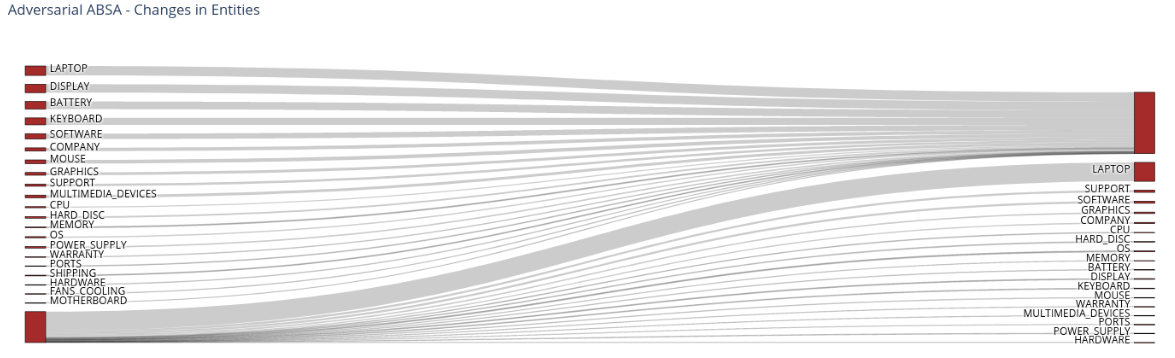
\includegraphics[ width = 1\textwidth]{img/entity_leet.png}
    \caption{Changes in entities - Attack Method: Leet Speak. Note that only results are displayed that have been changed and the ones that stay are hidden.}
    \label{fig:entity_leet}
\end{figure}


In Figure~\ref{fig:entity_attr_leet}, we analyze the change of entity-attribute sets caused by the perturbation through leet speak. The attributes removed most often are GENERAL, QUALITY, and OPERATION\textunderscore PERFORMANCE. The attributes most often falsely predicted after perturbation are QUALITY, GENERAL, and DESIGN\textunderscore FEATURES.

\begin{figure}
    \centering
    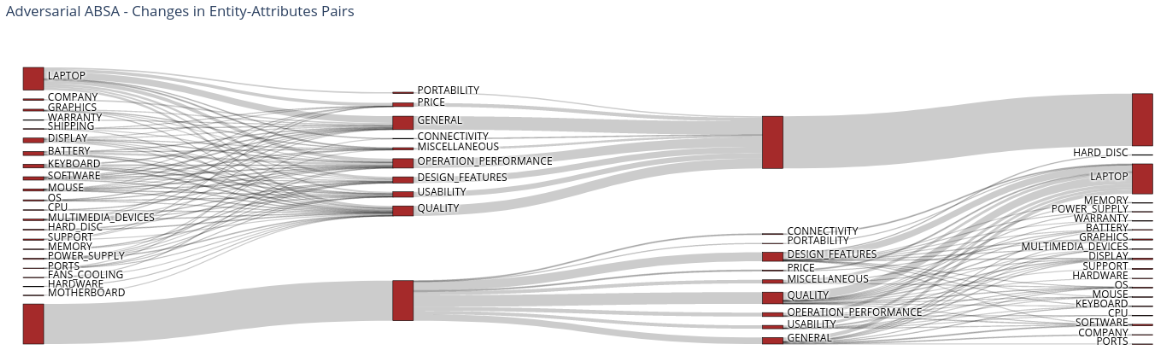
\includegraphics[ width = 1\textwidth]{img/entity_asp_leet.png}
    \caption{Changes in entity-attribute pairs - Attack Method: Leet Speak. Note that only results are displayed that have been changed and the ones that stay are hidden.}
    \label{fig:entity_attr_leet}
\end{figure}

In figure~\ref{fig:entity_attr_sent_leet}, we explore the flip of the entity-attribute sentiment set triggered by modifying a sentence using leat speak. The illustration shows that positive reviews are slightly less likely to be classified as such, while more reviews are falsely classified as negative when they are not.

\begin{figure}
    \centering
    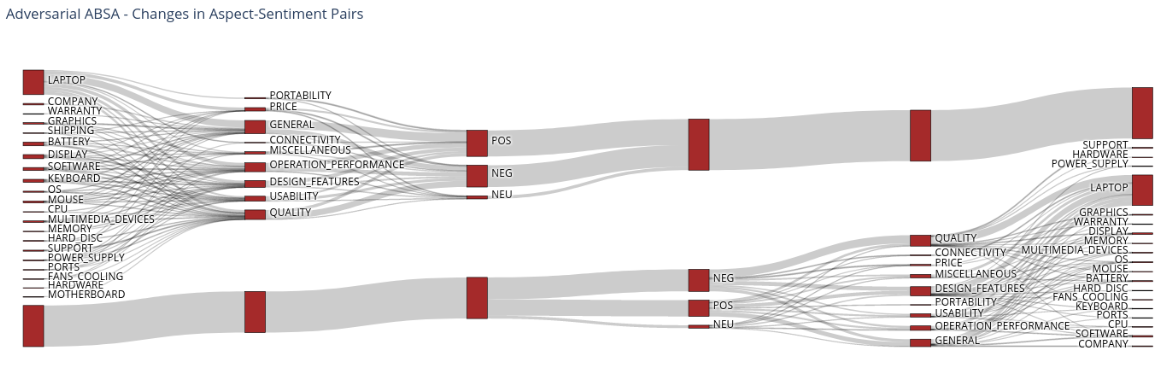
\includegraphics[ width = 1\textwidth]{img/entity_asp_sent_leet.png}
    \caption{Changes in entity-attribute sentiment sets - Attack Method: Leet Speak. Note that only results are displayed that have been changed and the ones that stay are hidden.}
    \label{fig:entity_attr_sent_leet}
\end{figure}

\textbf{Misspellings}

When only looking at the entities in figure~\ref{fig:entity_typo}, we see that SOFTWARE, SUPPORT, and OS were removed most often, whereas LAPTOP and COMPANY are much more likely to be added than other entities.

\begin{figure}
    \centering
    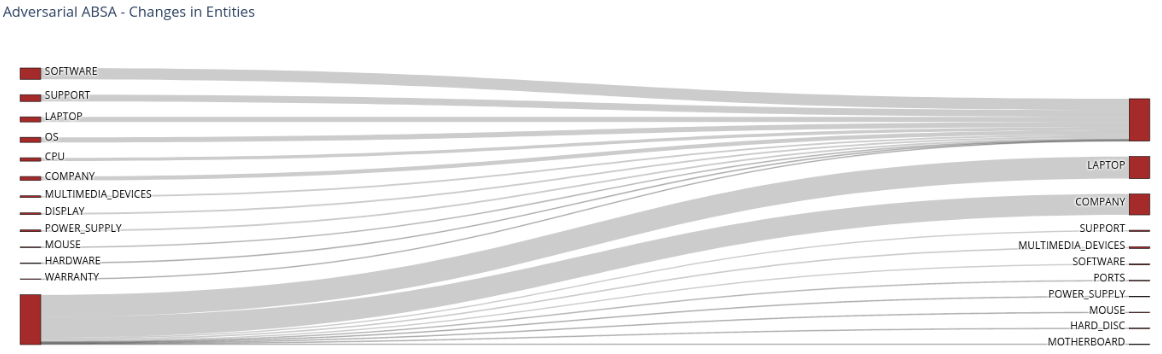
\includegraphics[ width = 1\textwidth]{img/entity_typo.png}
    \caption{Changes in entities - Attack Method: Misspellings. Note that only results are displayed that have been changed and the ones that stay are hidden.}
    \label{fig:entity_typo}
\end{figure}


When analyzing figure~\ref{fig:entity_attr_typo}, the entity-attribute sets flipped by the use of the misspellings, the attributes most often removed are GENERAL, QUALITY and OPERATION\textunderscore PERFORMANCE, while the most often added attributes are GENERAL, QUALITY, MISCELLANEOUS and DESIGN\textunderscore FEATURES.

\begin{figure}
    \centering
    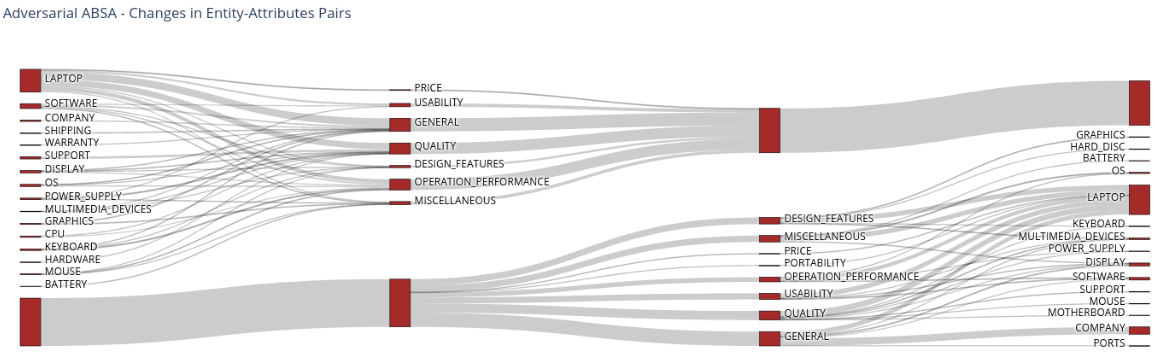
\includegraphics[ width = 1\textwidth]{img/entity_asp_typo.png}
    \caption{Changes in entity-attribute pairs - Attack Method: Misspellings. Note that only results are displayed that have been changed and the ones that stay are hidden.}
    \label{fig:entity_attr_typo}
\end{figure}

Figure~\ref{fig:entity_attr_sent_typo} shows that positive reviews are more likely to be not be classified as such through misspelling perturbations, while more reviews are falsely classified to be negative, while they are not.

\begin{figure}
    \centering
    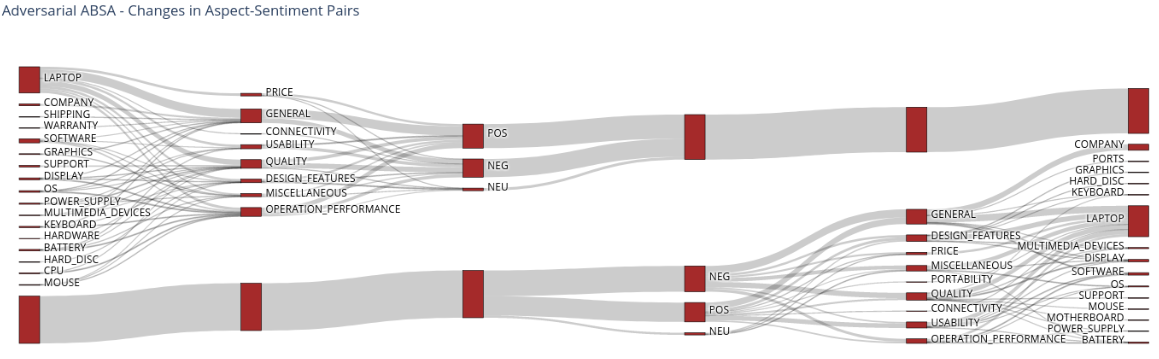
\includegraphics[ width = 1\textwidth]{img/entity_asp_sent_typo.png}
    \caption{Changes in entity-attribute sentiment sets - Attack Method: Misspellings. Note that only results are displayed that have been changed and the ones that stay are hidden.}
    \label{fig:entity_attr_sent_typo}
\end{figure}


\textbf{Punctuation}

Figure~\ref{fig:entity_punct} illustrates how the insertion of a punctuation mark after the determined important word reflects on the model's prediction of entities. We see that BATTERY, COMPANY, and LAPTOP were removed most often, whereas LAPTOP is remarkably more likely to be added than other entities. This means that content about the battery or the company is less likely to be detected in a sentence. Through adversarial punctuation, a sentence is more likely to be classified to contain information about a laptop or support subjects.

\begin{figure}
    \centering
    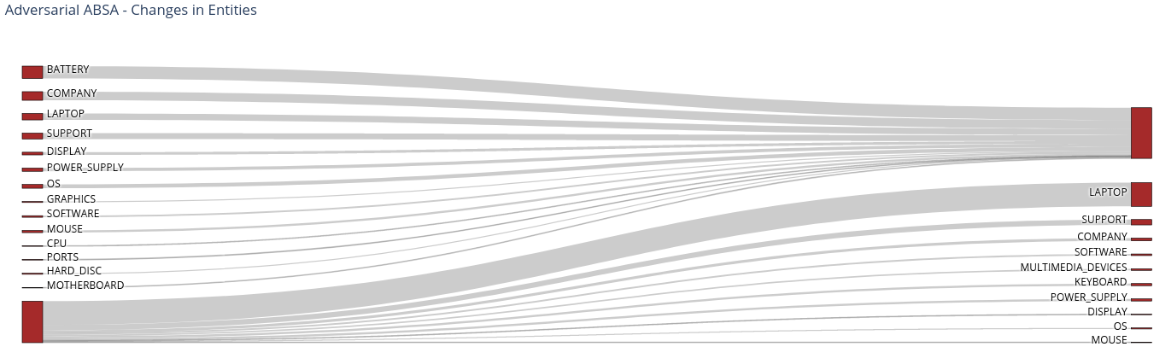
\includegraphics[ width = 1\textwidth]{img/entity_punct.png}
    \caption{Changes in entities - Attack Method: Punctuation. Note that only results are displayed that have been changed and the ones that stay are hidden.}
    \label{fig:entity_punct}
\end{figure}


In Figure~\ref{fig:entity_attr_punct}, we analyze the change of entity-attribute sets caused by inserting punctuation marks behind the important word. The attributes removed most often are QUALITY and OPERATION\textunderscore GENERAL. The attributes which were predicted for sentences, which do, in fact, not contain information about these attributes are QUALITY, GENERAL, and MISCELLANEOUS. 

\begin{figure}
    \centering
    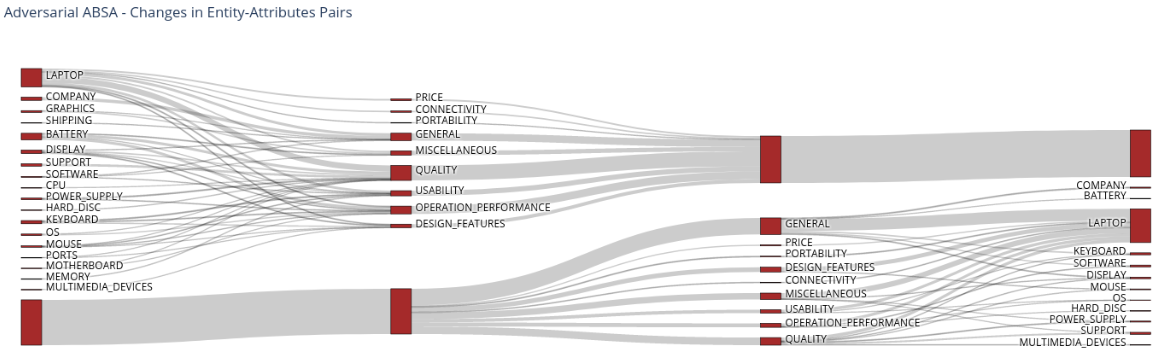
\includegraphics[ width = 1\textwidth]{img/entity_asp_punct.png}
    \caption{Changes in entity-attribute pairs - Attack Method: Punctuation. Note that only results are displayed that have been changed and the ones that stay are hidden.}
    \label{fig:entity_attr_punct}
\end{figure}

In figure~\ref{fig:entity_attr_sent_punct} we explore the flip of the entity-attribute sentiment set triggered through modifying a sentence using a additional punctuation mark. The figure illustrates that unlike the other two perturbation methods, positive reviews are slightly more likely to be classified as such. Like the two other methods, reviews were often falsely classified as negative when they are not.

\begin{figure}
    \centering
    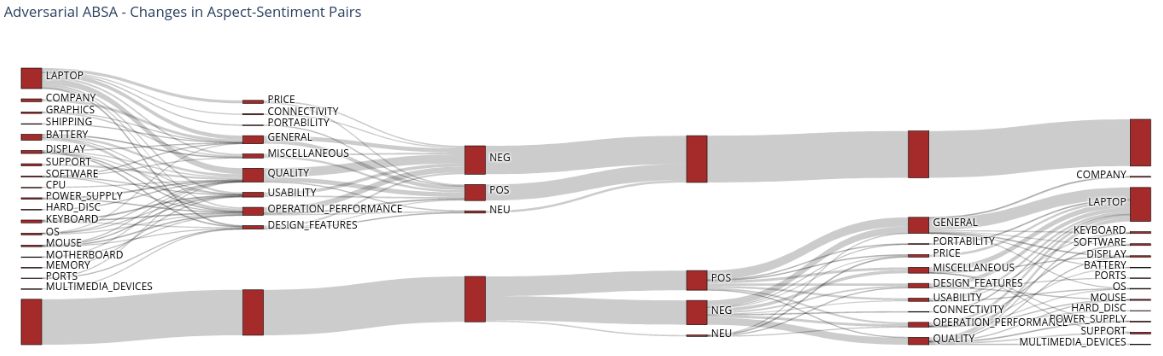
\includegraphics[ width = 1\textwidth]{img/entity_asp_sent_punct.png}
    \caption{Changes in entity-attribute sentiment sets - Attack Method: Punctuation. Note that only results are displayed that have been changed and the ones that stay are hidden.}
    \label{fig:entity_attr_sent_punct}
\end{figure}






\section{Discussion}
In a direct comparison we can see that the Leet Speak method has been the most successful. The least successful was the method of punctuation. This could be attributable to several reasons.

\subsection{Important Word Detection}

If we compare the results of the three methods in detail, we can see that in many cases the change of a word is decisive. 
This can best be demonstrated with an example. 
The result of the classification of the sentence "i love this notebook." is LAPTOP#GENERAL - POS. The important word identified by the LOO method is 'love'. If we use our Wikipedia typo dictionary, we find three ways to change the word. This results in the three modified sentences: "i lvoe this notebook.", "i loev this notebook.", and "i lveo this notebook.".
All three sentences result in the same false prediction:
"LAPTOP#MISCELLANEOUS" "NEG".

This indicates that it is not important how the important word is changed, but only that it has been changed and is therefore no longer recognized.
This effect could also be seen across methods:

Using the example in table ~\ref{tab:ex_sentence_gaming}, we see that regardless of the attack method, the entity attribute Sentiment set was incorrectly classified. 


\subsection{Word Embedding}
Let us recall the theory of word embedding of the BERT model:
BERT has a fixed set of learned word embeddings, composed in a word embedding lookup table, consisting of 30,522 words and word parts. 

To process sequences, BERT first transforms them into tokens. The token representation of the original sentence "It’s wonderful for computer gaming." is the following:


{[}CLS{]}  ||  it  ||  '  ||  s  ||  wonderful  ||  for  ||  computer  ||  gaming  ||  .  ||  {[}SEP{]} 


By changing the word 'wonderful' to w0nd3rfu1, as we do when attacking the model with the leed speak method, the token representation changes to:

{[}CLS{]}  ||  it  ||  '  ||  s  ||  w  ||  \#\#0  ||  \#\#nd  ||  \#\#3  ||  \#\#rf  ||  \#\#u  ||  \#\#1  ||  for  ||  computer  ||  gaming  ||  .  ||  {[}SEP{]}.

In this case BERT is no longer able to use the original word representation to assign semantic meaning to the word "wonderful", and will try to make sense of the remaining word pieces, being single letters, letter pairs and numbers.

We compare this with the second perturbation method, misspellings. The token representation of the sentences is the following:

{[}CLS{]}  ||  it  ||  '  ||  s  ||  wonderful  ||  \#\#l  ||  for  ||  computer  ||  gaming  ||  .  ||  {[}SEP{]}.

Note, that compared to the original token representation, only one extra token was added and all other token representations remain the same. It is therefore less challenging for the model, to still understand the sentence. Another aspect, why BERT should be more robust against the misspelling method is the corpus it is pre-trained on. To recall, the BERT model is pre-trained on all available Wikipedia articles. The dictionary we used for our experiments is a gathering of common typos found in wikipedia articles. BERT should therefore have assigned meaning to, at least some of the common typos.


In our third perturbation method, we added a comma after the important word "wonderful", resulting in a token representation looking like this:

{[}CLS{]}  ||  it  ||  '  ||  s  ||  wonderful  || , ||  for  ||  computer  ||  gaming  ||  .  ||  {[}SEP{]}.

There is still little literature available for the semantic representation of punctuation marks in BERT. In general, it can be said that it is difficult to attribute semantic meaning to a comma. Punctuation marks occur independently of context, sentiment, subject area and language style. Unlike, for example, the word "umbrella" which mostly occurs in the context of rain, this cannot be said about a comma. The only thing that recurs is that it usually occurs after the same words. For example after 'and' as well as at the beginning of sentences like 'Honestly', 'Lately' etc. But even these rules do not provide any information about the semantic meaning. This fact could be one explanation for the fact that the third method was not quite as effective as the perturbations through leet speak and misspellings.


\subsection{Attention}
In 


- meistens so, dass das veränderte Wort einfach nicht mehr erkannt wurde. Der Rest passt aber noch. Dadurch wurde die Attention auf was anderes gelegt. Der Rest bleibt gut.


generell meistens mehr aspecte gefunden durch modfication


\section{Conclusion, Limitations \& further Research}

\subsection{conclusion}
[exposé]
The idea is to implement the experiments in the running BERTbased ABSA Deep Learning Hotel Model of the company DeepOpinion. The model is already fine-tuned on user-generated reviews and trained on the ABSA text classification task. This gives me a head start, which limits the scope of my work. However, the model being the company's core technology, cannot be published in my thesis, which limits the reproducibility of my work.

%-------------------------------------------------------------------
%------------------------------Limitations -----------------------
%-------------------------------------------------------------------

\subsection{Limitations}

- other domains hotels and restaurants

%-------------------------------------------------------------------
%---------------------------Further Research -----------------------
%-------------------------------------------------------------------

\subsection{Further Research}

%END { system('cp', 'output.bbl', 'main.bbl'); }

% \nameref{Methodology}


%%% End:

\FloatBarrier


